% !TeX program = xelatex
% !TeX encoding = UTF-8
% Spedizione P05 · CO2: tendenza e calendario stagionale
% Presentazione della spedizione P05 nella serie planetaria di GeoStat Lab.
% Compilazione: xelatex -interaction=nonstopmode P05_CO2.tex (due passaggi)
% 32 slide. Diagrammi TikZ, figure vettoriali da R/P05_figure.R, codice R, dati ed esperimenti inclusi.
\RequirePackage{fix-cm}
\documentclass[12pt,aspectratio=1610]{beamer}
\geometry{paperwidth=20cm,paperheight=12.5cm}
\usepackage[italian,provide=*]{babel}
\usepackage{fontspec,adjustbox,tabularx}
\IfFontExistsTF{NimbusSans-Regular.otf}{
\setsansfont{NimbusSans-Regular.otf}[BoldFont=NimbusSans-Bold.otf,ItalicFont=NimbusSans-Italic.otf,BoldItalicFont=NimbusSans-BoldItalic.otf]
\setmainfont{NimbusSans-Regular.otf}[BoldFont=NimbusSans-Bold.otf,ItalicFont=NimbusSans-Italic.otf,BoldItalicFont=NimbusSans-BoldItalic.otf]
}{
\setsansfont{TeX Gyre Heros}
\setmainfont{TeX Gyre Heros}
}
\IfFontExistsTF{DejaVu Sans Mono}{
\setmonofont{DejaVu Sans Mono}[Scale=.88]
}{\setmonofont{Latin Modern Mono}[Scale=.88]}
\usefonttheme{professionalfonts}
\usepackage{amsmath,amssymb,booktabs,array,graphicx,tikz,bookmark}
\usetikzlibrary{calc,positioning,arrows.meta}
\graphicspath{{Figure/}}
\definecolor{Paper}{HTML}{F8F6F1}
\definecolor{Ink}{HTML}{253344}
\definecolor{Navy}{HTML}{15283E}
\definecolor{Quantum}{HTML}{5146A5}
\definecolor{Classical}{HTML}{087C74}
\definecolor{Muted}{HTML}{657180}
\definecolor{Rule}{HTML}{D6DAD9}
\definecolor{Night}{HTML}{112236}
\definecolor{Lilac}{HTML}{ABB5FF}
\definecolor{Mint}{HTML}{72D8C8}
\setbeamercolor{background canvas}{bg=Paper}
\setbeamercolor{normal text}{fg=Ink}
\setbeamertemplate{navigation symbols}{}
\setbeamertemplate{headline}{}
\setbeamertemplate{footline}{}
\setbeamersize{text margin left=0pt,text margin right=0pt}
\hypersetup{colorlinks=true,linkcolor=Classical,urlcolor=Classical,pdfpagemode=UseOutlines,pdfstartview=Fit,
 pdftitle={Spedizione P05 · CO2: tendenza e calendario stagionale},pdfauthor={GeoStat Lab · materiali di Marzio De Corato},
 pdfsubject={GeoStat Lab · P05}}
\bookmarksetup{open,openlevel=0,depth=2}
\newsavebox{\BodyBox}
\newsavebox{\SideBox}
\newsavebox{\RecallBox}
\newsavebox{\TitleBox}
\newcommand{\MeasureBox}[2]{\typeout{REVIEWBOX:#1:\the\wd#2:\the\ht#2:\the\dp#2}}

% Revisione completa: diagrammi TikZ, formalismo e box R.
\usepackage[most]{tcolorbox}
\usepackage{listings}
\usetikzlibrary{fit,backgrounds,matrix,decorations.pathreplacing}
\definecolor{GeoA}{HTML}{1D7890}
\definecolor{GeoB}{HTML}{C57E42}
\definecolor{GeoC}{HTML}{7363AA}
\definecolor{GeoTint}{HTML}{F0F4F3}
\lstdefinestyle{GeoR}{language=R,basicstyle=\ttfamily\fontsize{9.2}{12.2}\selectfont,
 keywordstyle=\color{Quantum}\bfseries,commentstyle=\color{Classical},stringstyle=\color{GeoB},
 numbers=left,numberstyle=\tiny\color{Muted},numbersep=4pt,showstringspaces=false,
 columns=fullflexible,keepspaces=true,breaklines=true,xleftmargin=1.15em,
 frame=none,aboveskip=0pt,belowskip=0pt,tabsize=2}
\newsavebox{\PilotLeftBox}
\newsavebox{\PilotRightBox}
\newcommand{\PLabel}[1]{\par{\color{Classical}\bfseries\fontsize{9}{11}\selectfont\MakeUppercase{#1}}\par\vspace{1.8mm}}
\newcommand{\PBody}[1]{\par{\fontsize{11.3}{14.8}\selectfont #1\par}}
\newcommand{\PSmall}[1]{\par{\fontsize{9.8}{13.1}\selectfont #1\par}}
\newcommand{\PCode}[2]{%
\begin{tcolorbox}[enhanced,arc=1.8mm,boxrule=.65pt,
  colback=white,colframe=Classical!75!Navy,colbacktitle=Navy,
  coltitle=white,fonttitle=\bfseries\fontsize{9.6}{12}\selectfont,
  title={#1},left=1.7mm,right=1.3mm,top=1.5mm,bottom=1.3mm,
  before skip=1mm,after skip=1mm]
\lstinputlisting[style=GeoR]{Codice/#2}
\end{tcolorbox}}
\newcommand{\PInfo}[1]{%
\begin{tcolorbox}[enhanced,arc=1.6mm,boxrule=.55pt,colback=GeoTint,
 colframe=Rule!80!Classical,left=2.3mm,right=2.3mm,top=2mm,bottom=2mm,
 before skip=1mm,after skip=1mm]
\PSmall{#1}\end{tcolorbox}}
\tikzset{
 pFlow/.style={draw=Classical!45,fill=white,rounded corners=2mm,
  line width=.7pt,align=center,minimum height=1.1cm,font=\sffamily\fontsize{10}{12}\selectfont},
 pEdge/.style={-{Latex[length=2.3mm]},draw=Classical,line width=.95pt},
 pGroup/.style={draw=Rule,fill=white,rounded corners=2mm,line width=.65pt},
 pDotA/.style={circle,fill=GeoA,inner sep=1.25pt},
 pDotB/.style={circle,fill=GeoB,inner sep=1.25pt},
 pDotC/.style={circle,fill=GeoC,inner sep=1.25pt}
}
\newcommand{\PilotChrome}[4]{%
  \node[anchor=north west,inner sep=0,text width=17.7cm] at ([xshift=.95cm,yshift=-.55cm]current page.north west) {\color{Navy}\bfseries\fontsize{20.6}{24.5}\selectfont #1};
  \node[anchor=north east,inner sep=0] at ([xshift=19.05cm,yshift=-.14cm]current page.north west) {\color{Classical}\fontsize{8}{10}\selectfont\hyperlink{slide2}{#2}};
  \draw[Classical,line width=1.2pt] ([xshift=.95cm,yshift=-1.7cm]current page.north west)--([xshift=2.35cm,yshift=-1.7cm]current page.north west);
  \draw[Rule,line width=.65pt] ([xshift=.95cm,yshift=-10.36cm]current page.north west)--([xshift=19.05cm,yshift=-10.36cm]current page.north west);
  \node[anchor=north west,inner sep=0] at ([xshift=.96cm,yshift=-10.55cm]current page.north west) {\color{Classical}\bfseries\fontsize{9.1}{12}\selectfont DA RICORDARE};
  \node[anchor=north west,inner sep=0,text width=14.3cm] at ([xshift=4.2cm,yshift=-10.53cm]current page.north west) {\color{Ink}\fontsize{10.3}{13.8}\selectfont #4};
  \draw[Rule,line width=.35pt] ([xshift=.95cm,yshift=-11.92cm]current page.north west)--([xshift=19.05cm,yshift=-11.92cm]current page.north west);
  \node[anchor=north west,inner sep=0] at ([xshift=.95cm,yshift=-12.06cm]current page.north west) {\color{Muted}\fontsize{7.7}{9.2}\selectfont Spedizione P05 · CO2: tendenza e calendario stagionale};
  \node[anchor=north east,inner sep=0] at ([xshift=19.05cm,yshift=-12.06cm]current page.north west) {\color{Muted}\fontsize{7.7}{9.2}\selectfont #3/32};
}


% Stili comuni per i diagrammi scientifici della revisione completa.
\tikzset{
 pAxis/.style={-{Latex[length=2mm]},draw=Muted,line width=.65pt},
 pNote/.style={font=\sffamily\fontsize{9}{11.5}\selectfont,text=Muted,align=center},
 pLabel/.style={font=\sffamily\fontsize{10}{12.5}\selectfont,text=Ink,align=center}
}
\newsavebox{\FullWideBox}
\setlength{\emergencystretch}{1em}




\newcommand{\PLab}[2]{\par{\color{Classical}\bfseries\fontsize{9}{11}\selectfont
\href{#1}{\MakeUppercase{#2}}}\par\vspace{1.8mm}}

\definecolor{Measure}{HTML}{A05B10}\definecolor{Rose}{HTML}{9B4564}\definecolor{Wash}{HTML}{EAE7F6}\definecolor{Gold}{HTML}{EEC184}
\tikzset{arr/.style={-{Stealth[length=2mm]},line width=.8pt,draw=Classical}}
\newcommand{\Colonna}[2]{\begin{adjustbox}{max totalsize={#1}{7.95cm},valign=t}\begin{minipage}[t]{#1}\raggedright\fontsize{11.3}{14.8}\selectfont #2\end{minipage}\end{adjustbox}}
\begin{document}

\begin{frame}[plain]\hypertarget{slide1}{}\bookmark[level=0,page=1]{Spedizione P05}
\begin{tikzpicture}[remember picture,overlay]
\fill[Night](current page.south west) rectangle(current page.north east);
\IfFileExists{Scena/copertina.jpg}{\node[inner sep=0] at(current page.center){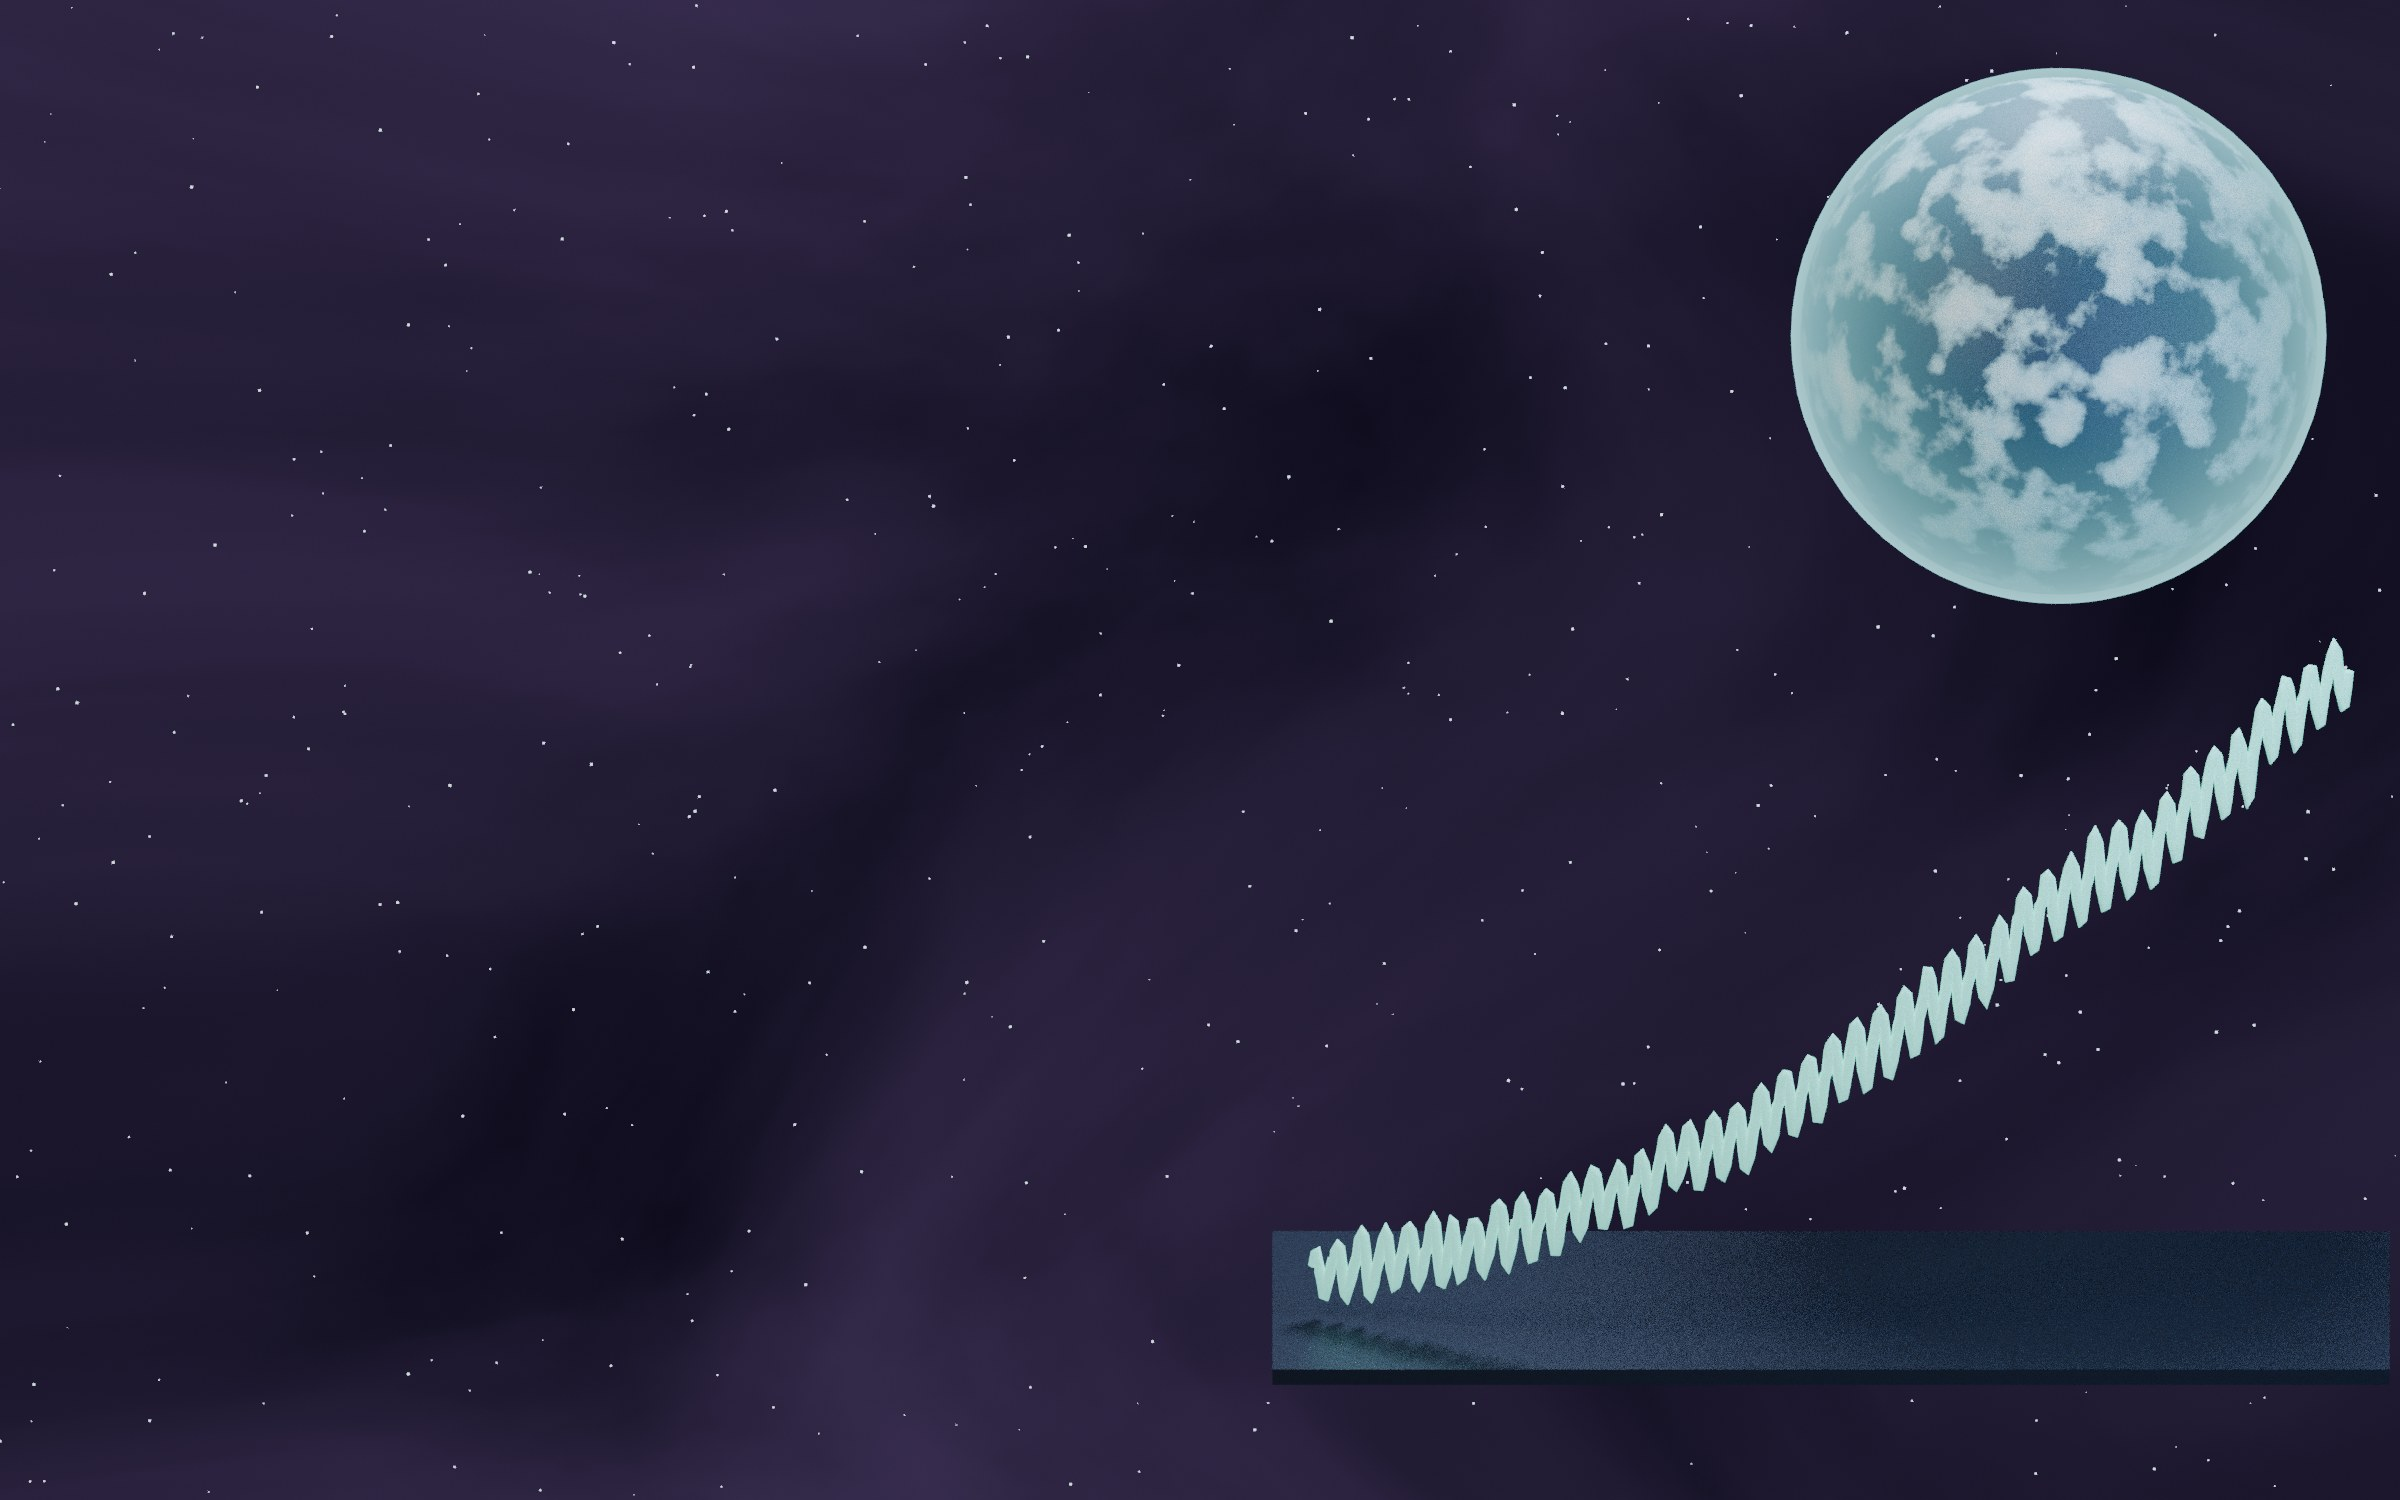
\includegraphics[width=20cm,height=12.5cm]{Scena/copertina.jpg}};}{}
\node[anchor=north west,inner sep=0] at([xshift=1.05cm,yshift=-1.10cm]current page.north west){\color{Mint}\bfseries\fontsize{23}{28}\selectfont SPEDIZIONE P05};
\node[anchor=north west,inner sep=0] at([xshift=1.07cm,yshift=-2.16cm]current page.north west){\color{white}\fontsize{9}{12}\selectfont MACROPROGETTO P05 · SCIENZE DELLA TERRA};
\draw[Mint,line width=1.5pt]([xshift=1.07cm,yshift=-2.78cm]current page.north west)--([xshift=2.6cm,yshift=-2.78cm]current page.north west);
\node[anchor=north west,inner sep=0] at([xshift=1.05cm,yshift=-3.35cm]current page.north west){\begin{minipage}{9.2cm}\raggedright\color{white}\bfseries\fontsize{28.5}{34.5}\selectfont CO$_2$: tendenza\\e calendario\\stagionale\end{minipage}};
\node[anchor=north west,inner sep=0] at([xshift=1.07cm,yshift=-7.88cm]current page.north west){\begin{minipage}{8.9cm}\raggedright\color{Lilac}\fontsize{12.2}{17}\selectfont Medie mensili a Mauna Loa, 1985–2000\end{minipage}};
\node[anchor=north west,inner sep=0] at([xshift=1.07cm,yshift=-8.70cm]current page.north west){\begin{minipage}{8.9cm}\raggedright\color{white!75}\fontsize{10.3}{14.5}\selectfont Medie mensili derivate, dipendenza residua e forma del trend\end{minipage}};
\node[anchor=north west,inner sep=0] at([xshift=1.07cm,yshift=-10.52cm]current page.north west){\color{white}\fontsize{10.5}{14}\selectfont GeoStat Lab · corso di Marzio De Corato};
\node[anchor=north west,inner sep=0] at([xshift=1.07cm,yshift=-11.17cm]current page.north west){\color{Mint}\fontsize{8.8}{11}\selectfont\href{https://creativecommons.org/licenses/by-nc-sa/4.0/}{Impaginazione da Tessera · CC BY-NC-SA 4.0}};
\end{tikzpicture}\end{frame}

\begin{frame}[plain]\hypertarget{slide2}{}
\bookmark[level=1,page=2]{Indice della presentazione}
\begin{tikzpicture}[remember picture,overlay]
\PilotChrome{Indice della presentazione}{PERCORSO}{2}{I titoli dell’indice aprono i capitoli. Il nome del capitolo in alto riporta a questa pagina.}
\node[anchor=north west,inner sep=0] at([xshift=.96cm,yshift=-2.12cm]current page.north west){\Colonna{9.40cm}{\PLabel{Capitoli}
{\fontsize{10.7}{13.5}\selectfont\hyperlink{slide4}{Provenienza e aggregazione della serie\hfill 4}\par}\vspace{.16cm}
{\fontsize{10.7}{13.5}\selectfont\hyperlink{slide9}{Scale temporali e modello della media\hfill 9}\par}\vspace{.16cm}
{\fontsize{10.7}{13.5}\selectfont\hyperlink{slide15}{Dipendenza e incertezza della pendenza\hfill 15}\par}\vspace{.16cm}
{\fontsize{10.7}{13.5}\selectfont\hyperlink{slide20}{Curvatura, interpretazione e consegna\hfill 20}\par}\vspace{.16cm}
{\fontsize{10.7}{13.5}\selectfont\hyperlink{slide24}{Laboratori della spedizione\hfill 24}\par}\vspace{.16cm}

}};
\node[anchor=north west,inner sep=0] at([xshift=10.85cm,yshift=-2.12cm]current page.north west){\Colonna{8.16cm}{\PLabel{Percorso di lettura}
\PBody{Il percorso ricostruisce la provenienza e l’aggregazione della serie, separa le scale temporali nel modello della media, misura la dipendenza dei residui e discute la forma del trend. I laboratori finali riprendono le tre fasi della spedizione.}
\PInfo{Le pagine Scenario A e Confronto riprendono gli esperimenti nel browser con dati sintetici. I valori di partenza del simulatore differiscono da quelli del caso.}
\href{https://marzione00.github.io/Lab_Geo/\#modulo-P05}{\color{Classical}\bfseries Apri la spedizione P05 su GeoStat Lab}
}};
\end{tikzpicture}\end{frame}

\begin{frame}[plain]\hypertarget{slide3}{}
\bookmark[level=1,page=3]{Quale tendenza si stima a Mauna Loa fra il 1985 e il 2000, al netto del calendario stagionale?}
\begin{tikzpicture}[remember picture,overlay]
\PilotChrome{{\fontsize{15.3}{19}\selectfont Quale tendenza si stima a Mauna Loa fra il 1985 e il 2000, al netto del calendario stagionale?}}{IL CASO GUIDA}{3}{La copertina è una scena illustrativa: il tubo luminoso segue le medie mensili della serie storica.}
\node[anchor=north west,inner sep=0] at([xshift=.96cm,yshift=-2.12cm]current page.north west){\Colonna{9.40cm}{{\centering\resizebox{0.97\linewidth}{!}{\begin{tikzpicture}[x=1cm,y=1cm,every node/.style={font=\sffamily\fontsize{10}{12}\selectfont,text=Ink}]
\draw[draw=Classical,fill=Classical!8,rounded corners=2mm,line width=.7pt] (0,0.00) rectangle (8.6,-0.78);
\node[circle,anchor=center,fill=Classical,inner sep=0,minimum size=.5cm,text=white,font=\sffamily\bfseries\fontsize{9}{10}\selectfont] at (.48,-0.39) {1};
\node[anchor=west,text width=7.4cm,align=left] at (.95,-0.39) {Provenienza e aggregazione della serie};
\draw[pEdge] (.48,-0.80)--(.48,-1.02);
\draw[draw=Classical,fill=Classical!8,rounded corners=2mm,line width=.7pt] (0,-1.04) rectangle (8.6,-1.82);
\node[circle,anchor=center,fill=Classical,inner sep=0,minimum size=.5cm,text=white,font=\sffamily\bfseries\fontsize{9}{10}\selectfont] at (.48,-1.43) {2};
\node[anchor=west,text width=7.4cm,align=left] at (.95,-1.43) {Scale temporali e modello della media};
\draw[pEdge] (.48,-1.84)--(.48,-2.06);
\draw[draw=Classical,fill=Classical!8,rounded corners=2mm,line width=.7pt] (0,-2.08) rectangle (8.6,-2.86);
\node[circle,anchor=center,fill=Classical,inner sep=0,minimum size=.5cm,text=white,font=\sffamily\bfseries\fontsize{9}{10}\selectfont] at (.48,-2.47) {3};
\node[anchor=west,text width=7.4cm,align=left] at (.95,-2.47) {Dipendenza e incertezza della pendenza};
\draw[pEdge] (.48,-2.88)--(.48,-3.10);
\draw[draw=Classical,fill=Classical!8,rounded corners=2mm,line width=.7pt] (0,-3.12) rectangle (8.6,-3.90);
\node[circle,anchor=center,fill=Classical,inner sep=0,minimum size=.5cm,text=white,font=\sffamily\bfseries\fontsize{9}{10}\selectfont] at (.48,-3.51) {4};
\node[anchor=west,text width=7.4cm,align=left] at (.95,-3.51) {Curvatura, interpretazione e consegna};
\draw[pEdge] (.48,-3.92)--(.48,-4.14);
\draw[draw=GeoB,fill=GeoB!8,rounded corners=2mm,line width=.7pt] (0,-4.16) rectangle (8.6,-4.94);
\node[circle,anchor=center,fill=GeoB,inner sep=0,minimum size=.5cm,text=white,font=\sffamily\bfseries\fontsize{9}{10}\selectfont] at (.48,-4.55) {L};
\node[anchor=west,text width=7.4cm,align=left] at (.95,-4.55) {Laboratori della spedizione};
\end{tikzpicture}
}\par}
\PSmall{Capitoli della spedizione; L indica i laboratori conclusivi.}
}};
\node[anchor=north west,inner sep=0] at([xshift=10.85cm,yshift=-2.12cm]current page.north west){\Colonna{8.16cm}{\PLabel{Il caso}
\PBody{Medie mensili derivate da osservazioni settimanali storiche della CO$_2$ a Mauna Loa, attribuite a Keeling e Whorf, coprono la finestra 1985–2000. Il modello separa una componente lineare da undici contrasti mensili e ne esamina i residui.}
\PInfo{Seguiremo la pendenza dall’intervallo classico a quello HAC, poi la curvatura che rende variabile il tasso di crescita lungo la finestra.}
}};
\end{tikzpicture}\end{frame}

\begin{frame}[plain]\hypertarget{slide4}{}
\bookmark[level=0,page=4]{Provenienza e aggregazione della serie}
\bookmark[level=1,page=4]{Una tendenza entro una finestra storica definita}
\begin{tikzpicture}[remember picture,overlay]
\PilotChrome{Una tendenza entro una finestra storica definita}{PROVENIENZA E AGGREGAZIONE DELLA SERIE}{4}{Provenienza, aggregazione e finestra temporale definiscono l’oggetto della stima.}
\node[anchor=north west,inner sep=0] at([xshift=.96cm,yshift=-2.12cm]current page.north west){\Colonna{9.40cm}{{\centering\resizebox{0.90\linewidth}{!}{\begin{tikzpicture}[x=1cm,y=-.87cm,every node/.style={font=\fontsize{12.2}{15}\selectfont,text=Ink},arr/.style={-{Stealth[length=2mm]},line width=.8pt,draw=Classical}]\path[use as bounding box] (0,0) rectangle (7.45,6.2);
\draw[draw=Classical,fill=Classical!8,rounded corners=2pt,line width=.7pt] (0.5,0.5) rectangle (6.9,1.8);
\node[anchor=center,text=Ink,font=\fontsize{11.5}{15}\selectfont,text width=6cm,align=center] at (3.7,1.15) {Serie settimanale storica conservata};
\draw[arr,draw=Classical] (3.7,2)--(3.7,2.6);
\draw[draw=Quantum,fill=Quantum!8,rounded corners=2pt,line width=.7pt] (0.5,2.8) rectangle (6.9,4.1);
\node[anchor=center,text=Ink,font=\fontsize{11.5}{15}\selectfont,text width=6cm,align=center] at (3.7,3.45) {Medie mensili e conteggio della copertura};
\draw[arr,draw=Classical] (3.7,4.3)--(3.7,4.9);
\node[anchor=center,text=Ink,font=\fontsize{12}{15}\selectfont,text width=6.7cm,align=center] at (3.7,5.5) {Finestra di analisi: 1985–2000};

\end{tikzpicture}}\par}
}};
\node[anchor=north west,inner sep=0] at([xshift=10.85cm,yshift=-2.12cm]current page.north west){\Colonna{8.16cm}{\PBody{Il progetto stima la tendenza della CO$_2$ a Mauna Loa nella finestra 1985–2000, utilizzando medie mensili derivate da osservazioni settimanali storiche distribuite con statsmodels. La fonte attribuisce la serie a Keeling e Whorf, attraverso CDIAC, e conserva il periodo fino al 2001. La domanda distingue una componente lineare e un calendario stagionale medio, esaminando poi la dipendenza rimasta nei residui. Il risultato riguarda questa finestra e questa aggregazione, mentre un aggiornamento richiederebbe la ricostruzione del protocollo su dati ufficiali nuovi.}
}};
\end{tikzpicture}\end{frame}

\begin{frame}[plain]\hypertarget{slide5}{}
\bookmark[level=1,page=5]{L’archivio distingue righe e osservazioni disponibili}
\begin{tikzpicture}[remember picture,overlay]
\PilotChrome{{\fontsize{15.3}{19}\selectfont L’archivio distingue righe e osservazioni disponibili}}{PROVENIENZA E AGGREGAZIONE DELLA SERIE}{5}{Il conteggio dei dati disponibili accompagna la sintesi numerica e ne chiarisce il supporto osservativo.}
\node[anchor=north west,inner sep=0] at([xshift=.96cm,yshift=-2.12cm]current page.north west){\Colonna{9.40cm}{\PBody{Il file conserva 2284 date settimanali, delle quali 59 hanno concentrazione mancante; i valori disponibili sono quindi 2225. La regolarità delle date e l’unicità delle righe vengono verificate prima dell’aggregazione. Una data presente con valore mancante mantiene informazione sulla copertura e non viene trasformata in concentrazione nulla. L’audit considera anche il periodo 1980–1984, precedente alla finestra finale, così che la selezione temporale e le lacune che la motivano rimangano documentate nell’intero procedimento.}
\par\smallskip{\centering\adjustbox{max width=.98\linewidth}{$\displaystyle n_{righe}=2284,\qquad n_{validi}=2284-59=2225$}\par\smallskip}
}};
\node[anchor=north west,inner sep=0] at([xshift=10.85cm,yshift=-2.12cm]current page.north west){\Colonna{8.16cm}{\PInfo{La serie mensile costruita nel progetto è una media delle settimane disponibili assegnate al mese dalla loro data. Essa va distinta da un prodotto mensile ufficiale ottenuto con altri protocolli di campionamento, controllo e ponderazione temporale.}
}};
\end{tikzpicture}\end{frame}

\begin{frame}[plain]\hypertarget{slide6}{}
\bookmark[level=1,page=6]{La media mensile mantiene il proprio denominatore}
\begin{tikzpicture}[remember picture,overlay]
\PilotChrome{La media mensile mantiene il proprio denominatore}{PROVENIENZA E AGGREGAZIONE DELLA SERIE}{6}{Una media derivata deve conservare la regola di selezione e il numero dei contributi effettivi.}
\node[anchor=north west,inner sep=0] at([xshift=.96cm,yshift=-2.12cm]current page.north west){\Colonna{9.40cm}{{\centering\resizebox{0.90\linewidth}{!}{\begin{tikzpicture}[x=1cm,y=-.87cm,every node/.style={font=\fontsize{12.2}{15}\selectfont,text=Ink},arr/.style={-{Stealth[length=2mm]},line width=.8pt,draw=Classical}]\path[use as bounding box] (0,0) rectangle (7.45,6.2);
\draw[draw=Classical,fill=Classical!8,rounded corners=2pt,line width=.7pt] (0.6,1.1) rectangle (1.8,2.3);
\node[anchor=center,text=Ink,font=\fontsize{13}{15}\selectfont] at (1.2,1.7) {1};
\draw[draw=Classical,fill=Classical!8,rounded corners=2pt,line width=.7pt] (2.2,1.1) rectangle (3.4000000000000004,2.3);
\node[anchor=center,text=Ink,font=\fontsize{13}{15}\selectfont] at (2.8,1.7) {2};
\draw[draw=Rule,fill=Rule!8,rounded corners=2pt,line width=.7pt] (3.8000000000000003,1.1) rectangle (5.0,2.3);
\node[anchor=center,text=Ink,font=\fontsize{13}{15}\selectfont] at (4.4,1.7) {NA};
\draw[draw=Classical,fill=Classical!8,rounded corners=2pt,line width=.7pt] (5.4,1.1) rectangle (6.6000000000000005,2.3);
\node[anchor=center,text=Ink,font=\fontsize{13}{15}\selectfont] at (6.000000000000001,1.7) {4};
\draw[arr,draw=Classical] (3.6,2.6)--(3.6,3.5);
\draw[draw=Quantum,fill=Quantum!8,rounded corners=2pt,line width=.7pt] (0.7,3.7) rectangle (6.6,5.1);
\node[anchor=center,text=Ink,font=\fontsize{12}{15}\selectfont,text width=5.5cm,align=center] at (3.65,4.4) {Media di tre valori disponibili};
\node[anchor=center,text=Ink,font=\fontsize{10.5}{15}\selectfont,text width=6.8cm,align=center] at (3.7,5.9) {Schema: il valore mancante resta escluso dalla somma.};

\end{tikzpicture}}\par}
\PSmall{$O_m$: settimane valide assegnate al mese m; $C_w$: concentrazione settimanale in ppm; $n_m$: numero dei contributi.}
}};
\node[anchor=north west,inner sep=0] at([xshift=10.85cm,yshift=-2.12cm]current page.north west){\Colonna{8.16cm}{\PBody{Per ogni mese si calcola la media aritmetica delle concentrazioni settimanali disponibili e si registra il numero dei contributi. Il procedimento assegna uguale peso alle settimane osservate, senza interpolare quelle assenti. Una media pesata per giorni effettivamente coperti richiederebbe metadati e una convenzione differente. L’analisi seleziona i 192 mesi del 1985–2000, per i quali il numero di settimane valide è almeno tre, mantenendo esplicito il criterio di copertura applicato alla finestra.}
\par\smallskip{\centering\adjustbox{max width=.98\linewidth}{$\displaystyle \overline C_m=\frac1{n_m}\sum_{w\in O_m}C_w,\qquad n_m=|O_m|\geq3$}\par\smallskip}
}};
\end{tikzpicture}\end{frame}

\begin{frame}[plain]\hypertarget{slide7}{}
\bookmark[level=1,page=7]{La copertura viene calcolata prima della selezione}
\begin{tikzpicture}[remember picture,overlay]
\PilotChrome{La copertura viene calcolata prima della selezione}{PROVENIENZA E AGGREGAZIONE DELLA SERIE}{7}{Il criterio di copertura viene applicato a una tabella che conserva sia la sintesi sia il denominatore.}
\node[anchor=north west,inner sep=0] at([xshift=.96cm,yshift=-2.12cm]current page.north west){\Colonna{9.40cm}{\PBody{Il frammento costruisce separatamente le medie e i conteggi, riunendoli mediante il mese. L’unione conserva anche eventuali mesi privi di media, che resterebbero riconoscibili attraverso il conteggio nullo. La finestra viene poi selezionata con estremi dichiarati e verificata rispetto al requisito delle tre settimane. Questa sequenza rende l’aggregazione controllabile e impedisce che una media numericamente definita nasconda un supporto temporale insufficiente per la comparabilità richiesta dall’analisi.}
}};
\node[anchor=north west,inner sep=0] at([xshift=10.85cm,yshift=-2.12cm]current page.north west){\Colonna{8.16cm}{\begin{tcolorbox}[enhanced,arc=1.7mm,boxrule=.6pt,colback=white,colframe=Classical!60!Navy,colbacktitle=Navy,coltitle=white,fonttitle=\bfseries\small,title={R · calcolo riproducibile},left=1.7mm,right=1.3mm,top=1.1mm,bottom=1.1mm,before skip=1mm,after skip=1.0mm]\lstinputlisting[style=GeoR,language=R,basicstyle=\ttfamily\fontsize{8.6}{11.4}\selectfont]{Codice/aggregazione.R}\end{tcolorbox}
\PLabel{Risultato in R}
\begin{tcolorbox}[colback=GeoTint,colframe=Rule,boxrule=.5pt,arc=1.4mm,left=2mm,right=1mm,top=1mm,bottom=1mm]{\fontsize{8.4}{10.9}\selectfont\ttfamily \mbox{}\\\mbox{\ \ 4\ \ \ 5\ }\\\mbox{126\ \ 66\ }}\end{tcolorbox}
}};
\end{tikzpicture}\end{frame}

\begin{frame}[plain]\hypertarget{slide8}{}
\bookmark[level=1,page=8]{L’audit rende visibile il mese scarsamente coperto}
\begin{tikzpicture}[remember picture,overlay]
\PilotChrome{L’audit rende visibile il mese scarsamente coperto}{PROVENIENZA E AGGREGAZIONE DELLA SERIE}{8}{La qualità della copertura va resa leggibile anche fuori dalla finestra infine utilizzata.}
\node[anchor=north west,inner sep=0] at([xshift=.96cm,yshift=-2.12cm]current page.north west){\Colonna{9.40cm}{{\centering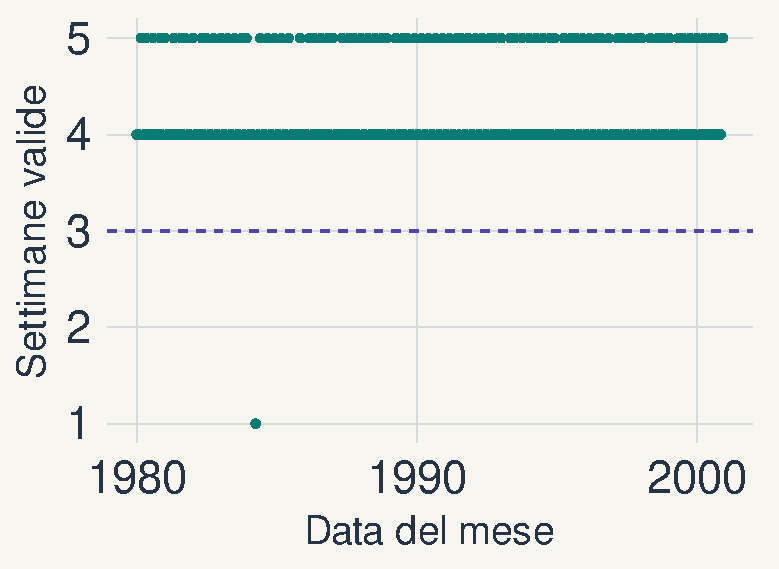
\includegraphics[width=\linewidth,height=6.15cm,keepaspectratio]{Figure/F01.pdf}\par}
\PSmall{Settimane valide per mese dal 1980 al 2000. Riferimento viola: criterio minimo di tre contributi.}
}};
\node[anchor=north west,inner sep=0] at([xshift=10.85cm,yshift=-2.12cm]current page.north west){\Colonna{8.16cm}{\PBody{Nel periodo più ampio 1980–2000, aprile 1984 contiene soltanto una settimana valida. La figura conserva questo mese e gli altri conteggi, insieme alla soglia di tre contributi richiesta nella finestra finale. La presenza di una media per aprile non garantirebbe quindi una copertura confrontabile con quella dei mesi successivi. La selezione 1985–2000 viene documentata attraverso questo controllo e non mediante una cancellazione silenziosa delle osservazioni problematiche dall’archivio originale.}
}};
\end{tikzpicture}\end{frame}

\begin{frame}[plain]\hypertarget{slide9}{}
\bookmark[level=0,page=9]{Scale temporali e modello della media}
\bookmark[level=1,page=9]{La serie presenta crescita e oscillazione annuale}
\begin{tikzpicture}[remember picture,overlay]
\PilotChrome{La serie presenta crescita e oscillazione annuale}{SCALE TEMPORALI E MODELLO DELLA MEDIA}{9}{La separazione delle componenti temporali richiede ipotesi esplicite sulla forma della media.}
\node[anchor=north west,inner sep=0] at([xshift=.96cm,yshift=-2.12cm]current page.north west){\Colonna{9.40cm}{{\centering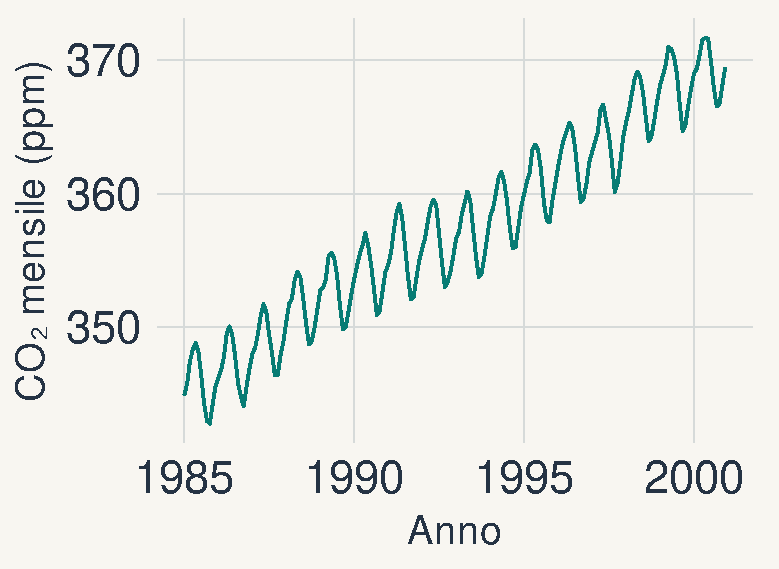
\includegraphics[width=\linewidth,height=6.15cm,keepaspectratio]{Figure/F02.pdf}\par}
\PSmall{Medie mensili derivate dalle settimane disponibili, gennaio 1985–dicembre 2000.}
}};
\node[anchor=north west,inner sep=0] at([xshift=10.85cm,yshift=-2.12cm]current page.north west){\Colonna{8.16cm}{\PBody{Le 192 medie mensili mostrano una crescita di lungo periodo sulla quale si sovrappone un’oscillazione stagionale. La rappresentazione temporale conserva entrambe le scale e permette di valutare se una tendenza lineare costituisca una sintesi ragionevole della finestra. La regolarità visiva del ciclo non implica che ampiezza e forma siano identiche in tutti gli anni. Il modello successivo assume un calendario medio, la cui adeguatezza verrà esaminata attraverso residui e sensibilità della forma della tendenza.}
}};
\end{tikzpicture}\end{frame}

\begin{frame}[plain]\hypertarget{slide10}{}
\bookmark[level=1,page=10]{Gli scarti annui isolano una descrizione stagionale}
\begin{tikzpicture}[remember picture,overlay]
\PilotChrome{{\fontsize{15.3}{19}\selectfont Gli scarti annui isolano una descrizione stagionale}}{SCALE TEMPORALI E MODELLO DELLA MEDIA}{10}{Una trasformazione descrittiva va distinta dalla risposta utilizzata nella stima del modello.}
\node[anchor=north west,inner sep=0] at([xshift=.96cm,yshift=-2.12cm]current page.north west){\Colonna{9.40cm}{{\centering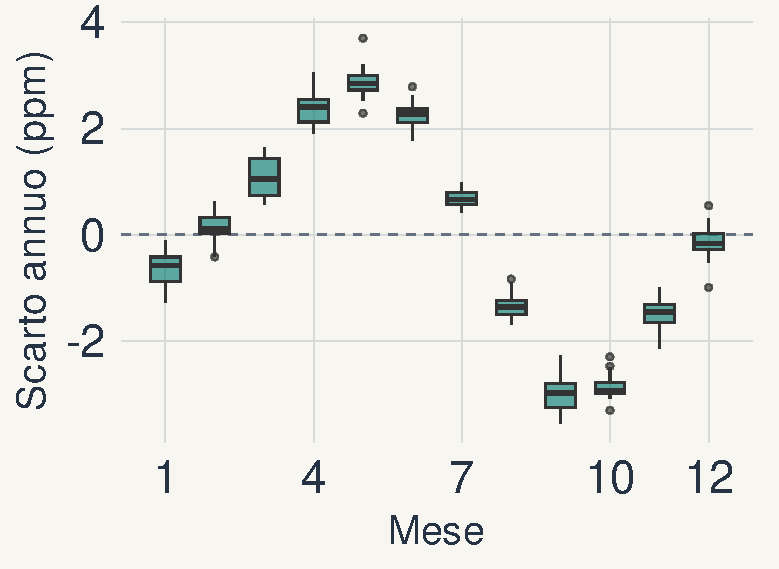
\includegraphics[width=\linewidth,height=6.15cm,keepaspectratio]{Figure/F03.pdf}\par}
\PSmall{$C_{y,m}$: media mensile nell’anno y e mese m; $A_{y,m}$: scarto dalla media annua, in ppm. Sedici valori per mese.}
}};
\node[anchor=north west,inner sep=0] at([xshift=10.85cm,yshift=-2.12cm]current page.north west){\Colonna{8.16cm}{\PBody{Sottraendo a ciascun mese la media del proprio anno si ottiene una descrizione della posizione stagionale relativa. I boxplot riuniscono, per ogni mese calendario, gli scarti osservati nei sedici anni della finestra. La dispersione delle scatole riguarda la variabilità fra anni e non l’incertezza della pendenza temporale. La trasformazione viene utilizzata soltanto per la visualizzazione, mentre il modello finale è stimato sulle concentrazioni mensili originarie, conservando la componente di crescita che la centratura annua rimuove.}
\par\smallskip{\centering\adjustbox{max width=.98\linewidth}{$\displaystyle A_{y,m}=C_{y,m}-\frac1{12}\sum_{j=1}^{12}C_{y,j}$}\par\smallskip}
}};
\end{tikzpicture}\end{frame}

\begin{frame}[plain]\hypertarget{slide11}{}
\bookmark[level=1,page=11]{Una pendenza e undici contrasti mensili}
\begin{tikzpicture}[remember picture,overlay]
\PilotChrome{Una pendenza e undici contrasti mensili}{SCALE TEMPORALI E MODELLO DELLA MEDIA}{11}{La categoria di riferimento e l’unità del tempo determinano il significato dei coefficienti.}
\node[anchor=north west,inner sep=0] at([xshift=.96cm,yshift=-2.12cm]current page.north west){\Colonna{9.40cm}{\PBody{Il modello associa alla concentrazione una tendenza lineare e undici effetti mensili, lasciando gennaio come categoria di riferimento. Il tempo viene espresso in anni e centrato rispetto al 1993, così che la pendenza abbia unità ppm per anno. L’intercetta riguarda il gennaio di riferimento al tempo centrato zero secondo la convenzione adottata. Gli effetti mensili descrivono differenze medie rispetto a gennaio, mentre la pendenza rappresenta una crescita comune al calendario stagionale mantenuto costante.}
\par\smallskip{\centering\adjustbox{max width=.98\linewidth}{$\displaystyle C_t=\alpha+\beta\tau_t+\sum_{m=2}^{12}\gamma_m\mathbf1\{M_t=m\}+\varepsilon_t$}\par\smallskip}
}};
\node[anchor=north west,inner sep=0] at([xshift=10.85cm,yshift=-2.12cm]current page.north west){\Colonna{8.16cm}{\PInfo{$C_t$: media mensile in ppm; $M_t$: mese, da 1 a 12; $\tau_t=\mathrm{anno}_t+(M_t-0,5)/12-1993$, in anni. $\alpha$: intercetta; $\beta$: pendenza; $\gamma_m$: contrasto con gennaio; $\varepsilon_t$: errore a media nulla. Si fissa $\gamma_1=0$. Le tredici colonne sono intercetta, tempo e undici indicatori; dodici indicatori più intercetta sarebbero ridondanti.}
}};
\end{tikzpicture}\end{frame}

\begin{frame}[plain]\hypertarget{slide12}{}
\bookmark[level=1,page=12]{Il rango esprime l’identificabilità dei coefficienti}
\begin{tikzpicture}[remember picture,overlay]
\PilotChrome{{\fontsize{15.3}{19}\selectfont Il rango esprime l’identificabilità dei coefficienti}}{SCALE TEMPORALI E MODELLO DELLA MEDIA}{12}{L’identificabilità dipende dalle relazioni fra colonne, oltre che dal numero delle osservazioni.}
\node[anchor=north west,inner sep=0] at([xshift=.96cm,yshift=-2.12cm]current page.north west){\Colonna{9.40cm}{{\centering\resizebox{0.90\linewidth}{!}{\begin{tikzpicture}[x=1cm,y=-.87cm,every node/.style={font=\fontsize{12.2}{15}\selectfont,text=Ink},arr/.style={-{Stealth[length=2mm]},line width=.8pt,draw=Classical}]\path[use as bounding box] (0,0) rectangle (7.45,6.2);
\draw[draw=Classical,fill=Classical!8,rounded corners=2pt,line width=.7pt] (0.4,0.7) rectangle (2.1,4.8);
\node[anchor=center,text=Ink,font=\fontsize{22}{15}\selectfont] at (1.25,2.75) {1};
\draw[draw=Quantum,fill=Quantum!8,rounded corners=2pt,line width=.7pt] (2.3,0.7) rectangle (4,4.8);
\node[anchor=center,text=Ink,font=\fontsize{22}{15}\selectfont] at (3.15,2.75) {$\tau$};
\draw[draw=Classical,fill=Classical!8,rounded corners=2pt,line width=.7pt] (4.2,0.7) rectangle (7,4.8);
\node[anchor=center,text=Ink,font=\fontsize{12}{15}\selectfont,text width=2.5cm,align=center] at (5.6,2.75) {11 contrasti mensili};
\node[anchor=center,text=Ink,font=\fontsize{12}{15}\selectfont,text width=6.7cm,align=center] at (3.7,5.7) {192 righe, 13 colonne indipendenti};

\end{tikzpicture}}\par}
\PSmall{X: matrice del modello; n = 192 mesi; k = 13 coefficienti. Il rango pieno consente una soluzione OLS unica.}
}};
\node[anchor=north west,inner sep=0] at([xshift=10.85cm,yshift=-2.12cm]current page.north west){\Colonna{8.16cm}{\PBody{La verifica del rango controlla che le colonne della matrice del modello forniscano informazioni linearmente distinte. La scelta di gennaio come riferimento elimina la ridondanza fra intercetta e indicatori mensili, rendendo identificabili i coefficienti nella parametrizzazione adottata. Cambiare il mese di riferimento modificherebbe intercetta e contrasti, lasciando invariati valori adattati e pendenza temporale. Questa equivalenza riguarda una ricodifica dello stesso spazio delle medie, mentre aggiungere una curvatura introdurrebbe uno spazio di modelli più ampio.}
\par\smallskip{\centering\adjustbox{max width=.98\linewidth}{$\displaystyle \operatorname{rank}(X)=13,\qquad n-k=192-13=179$}\par\smallskip}
}};
\end{tikzpicture}\end{frame}

\begin{frame}[plain]\hypertarget{slide13}{}
\bookmark[level=1,page=13]{La stima conserva la scala di ppm per anno}
\begin{tikzpicture}[remember picture,overlay]
\PilotChrome{La stima conserva la scala di ppm per anno}{SCALE TEMPORALI E MODELLO DELLA MEDIA}{13}{Una buona aderenza complessiva non stabilisce da sola la correttezza della covarianza degli errori.}
\node[anchor=north west,inner sep=0] at([xshift=.96cm,yshift=-2.12cm]current page.north west){\Colonna{9.40cm}{\PBody{La pendenza stimata è circa 1,53691 ppm per anno e il coefficiente di determinazione è circa 0,9909. Il primo valore riassume la crescita media nella specificazione lineare stagionale; il secondo descrive la quota di variabilità campionaria spiegata dal modello. Un valore elevato di R² è compatibile con residui fortemente correlati e con una forma della media ancora semplificata. L’interpretazione della precisione richiede quindi l’esame dell’ordine temporale e dell’autocorrelazione dei residui.}
}};
\node[anchor=north west,inner sep=0] at([xshift=10.85cm,yshift=-2.12cm]current page.north west){\Colonna{8.16cm}{\begin{tcolorbox}[enhanced,arc=1.7mm,boxrule=.6pt,colback=white,colframe=Classical!60!Navy,colbacktitle=Navy,coltitle=white,fonttitle=\bfseries\small,title={R · calcolo riproducibile},left=1.7mm,right=1.3mm,top=1.1mm,bottom=1.1mm,before skip=1mm,after skip=1.0mm]\lstinputlisting[style=GeoR,language=R,basicstyle=\ttfamily\fontsize{8.6}{11.4}\selectfont]{Codice/modello.R}\end{tcolorbox}
\PLabel{Risultato in R}
\begin{tcolorbox}[colback=GeoTint,colframe=Rule,boxrule=.5pt,arc=1.4mm,left=2mm,right=1mm,top=1mm,bottom=1mm]{\fontsize{8.4}{10.9}\selectfont\ttfamily \mbox{\ \ \ \ \ \ \ t\ }\\\mbox{1.536914\ }\\\mbox{\ \ \ 2.5\ \%\ \ \ 97.5\ \%\ }\\\mbox{1.514420\ 1.559407\ }}\end{tcolorbox}
}};
\end{tikzpicture}\end{frame}

\begin{frame}[plain]\hypertarget{slide14}{}
\bookmark[level=1,page=14]{L’adattamento viene confrontato con la serie}
\begin{tikzpicture}[remember picture,overlay]
\PilotChrome{L’adattamento viene confrontato con la serie}{SCALE TEMPORALI E MODELLO DELLA MEDIA}{14}{La scala del grafico determina quali scostamenti rimangano visibili nella diagnosi.}
\node[anchor=north west,inner sep=0] at([xshift=.96cm,yshift=-2.12cm]current page.north west){\Colonna{9.40cm}{{\centering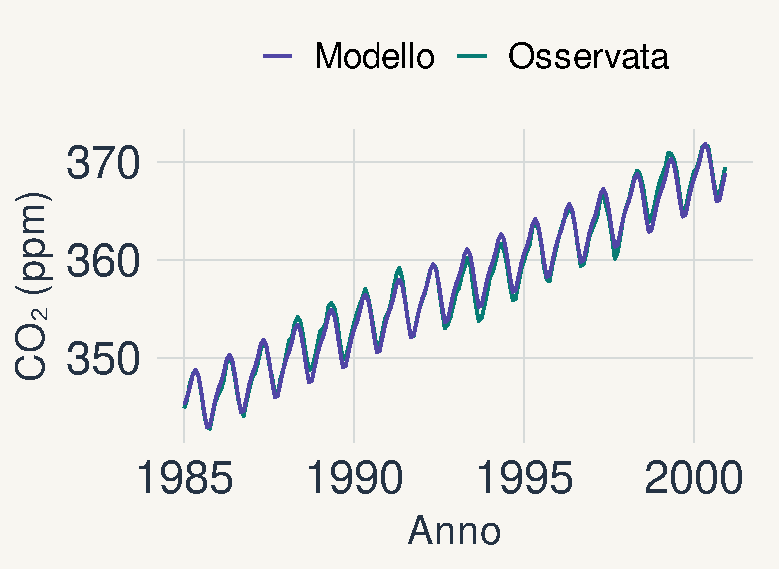
\includegraphics[width=\linewidth,height=6.15cm,keepaspectratio]{Figure/F04.pdf}\par}
\PSmall{Serie osservata e adattamento lineare con effetti mensili. Stessa scala e stessa finestra temporale.}
}};
\node[anchor=north west,inner sep=0] at([xshift=10.85cm,yshift=-2.12cm]current page.north west){\Colonna{8.16cm}{\PBody{Le concentrazioni osservate e quelle adattate vengono sovrapposte mantenendo la sequenza temporale. Il modello segue gran parte della crescita e dell’oscillazione annuale, mentre gli scarti residui risultano poco visibili nella scala complessiva della concentrazione. Per questo la sovrapposizione viene affiancata da un grafico dedicato ai residui, che ne amplia la scala. La scelta di due rappresentazioni consente di valutare sia l’aderenza globale sia le strutture più piccole che possono influenzare l’inferenza sul trend.}
}};
\end{tikzpicture}\end{frame}

\begin{frame}[plain]\hypertarget{slide15}{}
\bookmark[level=0,page=15]{Dipendenza e incertezza della pendenza}
\bookmark[level=1,page=15]{I residui conservano sequenze persistenti}
\begin{tikzpicture}[remember picture,overlay]
\PilotChrome{I residui conservano sequenze persistenti}{DIPENDENZA E INCERTEZZA DELLA PENDENZA}{15}{La persistenza residua va interpretata insieme alla possibilità di una media ancora incompletamente specificata.}
\node[anchor=north west,inner sep=0] at([xshift=.96cm,yshift=-2.12cm]current page.north west){\Colonna{9.40cm}{{\centering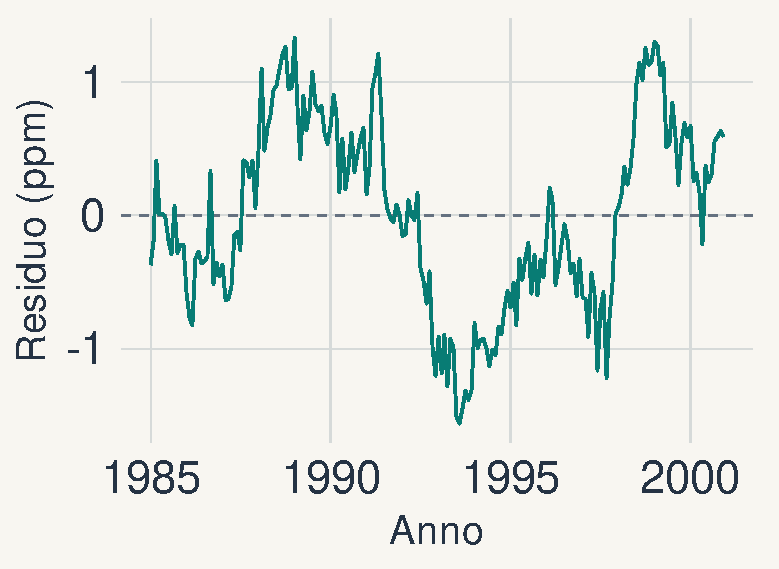
\includegraphics[width=\linewidth,height=6.15cm,keepaspectratio]{Figure/F05.pdf}\par}
\PSmall{Residui in ppm del modello lineare stagionale. La scala dedicata rende riconoscibili le sequenze temporali.}
}};
\node[anchor=north west,inner sep=0] at([xshift=10.85cm,yshift=-2.12cm]current page.north west){\Colonna{8.16cm}{\PBody{Gli scarti dalla media modellata mostrano periodi prolungati sopra o sotto lo zero, suggerendo una persistenza che la sola componente stagionale fissa lascia irrisolta. Questa struttura può riflettere dipendenza degli errori, variazioni della media omesse o entrambe. La rappresentazione temporale precede quindi il calcolo della covarianza robusta, poiché una correzione dell’errore standard non modifica la forma della tendenza. L’analisi mantiene distinti il problema della dipendenza e quello della specificazione del valore atteso.}
}};
\end{tikzpicture}\end{frame}

\begin{frame}[plain]\hypertarget{slide16}{}
\bookmark[level=1,page=16]{L’autocorrelazione rende esplicita la persistenza}
\begin{tikzpicture}[remember picture,overlay]
\PilotChrome{L’autocorrelazione rende esplicita la persistenza}{DIPENDENZA E INCERTEZZA DELLA PENDENZA}{16}{Una dipendenza residua pronunciata modifica l’informazione attribuibile alla sequenza delle osservazioni.}
\node[anchor=north west,inner sep=0] at([xshift=.96cm,yshift=-2.12cm]current page.north west){\Colonna{9.40cm}{{\centering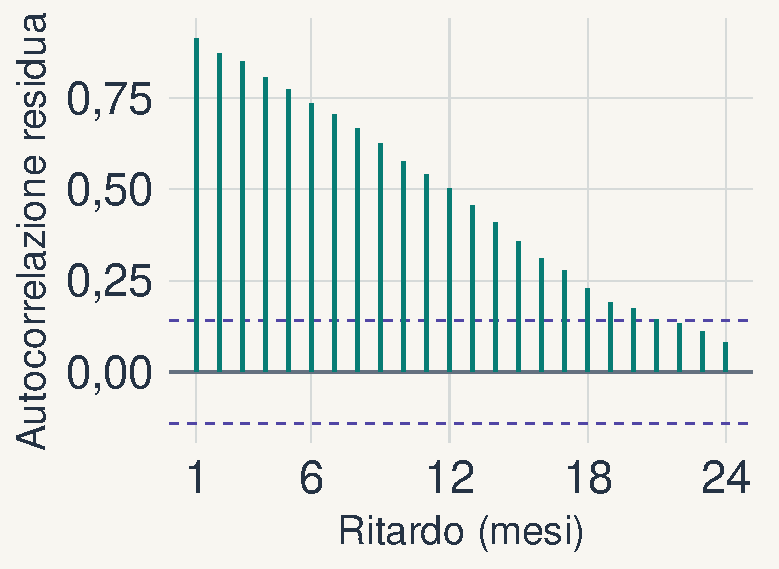
\includegraphics[width=\linewidth,height=6.15cm,keepaspectratio]{Figure/F06.pdf}\par}
\PSmall{ACF dei residui mensili. Bande puntuali approssimative pari a ±1,96 diviso la radice di 192.}
}};
\node[anchor=north west,inner sep=0] at([xshift=10.85cm,yshift=-2.12cm]current page.north west){\Colonna{8.16cm}{\PBody{L’ACF residua fino a ventiquattro mesi mostra una correlazione al primo ritardo di circa 0,914, che rende poco plausibile trattare gli scarti consecutivi come indipendenti. Le bande tratteggiate rappresentano il riferimento puntuale approssimativo di rumore bianco e non correggono il confronto simultaneo di tutte le barre. La persistenza sostiene l’esame di covarianze temporali e di modelli alternativi della media, mentre la sola posizione di una barra rispetto alla banda non identifica il meccanismo responsabile.}
}};
\end{tikzpicture}\end{frame}

\begin{frame}[plain]\hypertarget{slide17}{}
\bookmark[level=1,page=17]{L’intervallo HAC include prodotti temporali ritardati}
\begin{tikzpicture}[remember picture,overlay]
\PilotChrome{{\fontsize{15.3}{19}\selectfont L’intervallo HAC include prodotti temporali ritardati}}{DIPENDENZA E INCERTEZZA DELLA PENDENZA}{17}{La convenzione HAC comprende ritardo, pesi, correzione finita e riferimento asintotico.}
\node[anchor=north west,inner sep=0] at([xshift=.96cm,yshift=-2.12cm]current page.north west){\Colonna{9.40cm}{{\centering\resizebox{0.90\linewidth}{!}{\begin{tikzpicture}[x=1cm,y=-.87cm,every node/.style={font=\fontsize{12.2}{15}\selectfont,text=Ink},arr/.style={-{Stealth[length=2mm]},line width=.8pt,draw=Classical}]\path[use as bounding box] (0,0) rectangle (7.45,6.2);
\draw[draw=Classical,fill=Classical!8,rounded corners=2pt,line width=.7pt] (0.5,0.5) rectangle (6.9,1.8);
\node[anchor=center,text=Ink,font=\fontsize{11.5}{15}\selectfont,text width=6cm,align=center] at (3.7,1.15) {Residui ordinati e matrice del modello};
\draw[arr,draw=Classical] (3.7,2)--(3.7,2.6);
\draw[draw=Quantum,fill=Quantum!8,rounded corners=2pt,line width=.7pt] (0.5,2.8) rectangle (6.9,4.1);
\node[anchor=center,text=Ink,font=\fontsize{11.5}{15}\selectfont,text width=6cm,align=center] at (3.7,3.45) {Prodotti ritardati fino a dodici mesi};
\draw[arr,draw=Classical] (3.7,4.3)--(3.7,4.9);
\node[anchor=center,text=Ink,font=\fontsize{12}{15}\selectfont,text width=6.7cm,align=center] at (3.7,5.5) {Covarianza della pendenza stimata};

\end{tikzpicture}}\par}
\PSmall{X: 192 righe, colonne intercetta, tempo e 11 mesi; $S_{12}$: somma dei prodotti pesati regressore × residuo. L’elemento 22 riguarda la pendenza.}
}};
\node[anchor=north west,inner sep=0] at([xshift=10.85cm,yshift=-2.12cm]current page.north west){\Colonna{8.16cm}{\PBody{La covarianza HAC usa pesi di Bartlett fino a dodici mesi, senza prewhitening, e la correzione finita 192 diviso 179. La matrice interna combina prodotti fra residui e regressori, assegnando al ritardo h il peso uno meno h diviso tredici. L’errore standard deriva dalla diagonale della covarianza; l’intervallo usa il riferimento normale asintotico. La pendenza OLS resta invariata: cambia la stima dell’incertezza, sotto ipotesi di regolarità che la correzione finita non sostituisce.}
\par\smallskip{\centering\adjustbox{max width=.98\linewidth}{$\displaystyle \begin{gathered}\widehat V_{HAC}=\frac{192}{179}(X^TX)^{-1}S_{12}(X^TX)^{-1}\\IC_{HAC}=\widehat\beta\pm1{,}96\sqrt{[\widehat V_{HAC}]_{22}}\end{gathered}$}\par\smallskip}
}};
\end{tikzpicture}\end{frame}

\begin{frame}[plain]\hypertarget{slide18}{}
\bookmark[level=1,page=18]{La precisione cambia a stima invariata}
\begin{tikzpicture}[remember picture,overlay]
\PilotChrome{La precisione cambia a stima invariata}{DIPENDENZA E INCERTEZZA DELLA PENDENZA}{18}{La concordanza del segno può convivere con differenze sostanziali nella precisione dichiarata.}
\node[anchor=north west,inner sep=0] at([xshift=.96cm,yshift=-2.12cm]current page.north west){\Colonna{9.40cm}{{\centering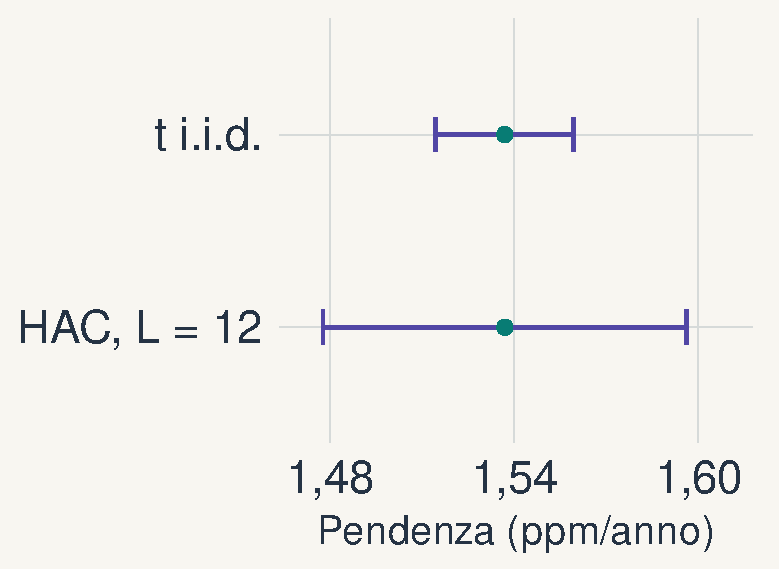
\includegraphics[width=\linewidth,height=6.15cm,keepaspectratio]{Figure/F10.pdf}\par}
\PSmall{Intervalli della stessa pendenza: t i.i.d. e normale HAC con L = 12. Unità: ppm per anno.}
}};
\node[anchor=north west,inner sep=0] at([xshift=10.85cm,yshift=-2.12cm]current page.north west){\Colonna{8.16cm}{\PBody{L’intervallo t i.i.d. della pendenza va da circa 1,51442 a 1,55941 ppm per anno, mentre quello HAC con dodici mesi va da circa 1,47762 a 1,59621. La seconda costruzione restituisce un’incertezza maggiore in questa serie, coerentemente con il contributo delle covarianze residue stimate. La crescita positiva rimane sostenuta nelle due specificazioni, ma la sua precisione differisce sensibilmente. Il confronto riguarda il modello adottato e non incorpora automaticamente l’incertezza su aggregazione, finestra o forma della media.}
}};
\end{tikzpicture}\end{frame}

\begin{frame}[plain]\hypertarget{slide19}{}
\bookmark[level=1,page=19]{La griglia dei ritardi rende verificabile la scelta}
\begin{tikzpicture}[remember picture,overlay]
\PilotChrome{{\fontsize{15.3}{19}\selectfont La griglia dei ritardi rende verificabile la scelta}}{DIPENDENZA E INCERTEZZA DELLA PENDENZA}{19}{La sensibilità della precisione viene documentata senza trasformare la griglia in una selezione del risultato.}
\node[anchor=north west,inner sep=0] at([xshift=.96cm,yshift=-2.12cm]current page.north west){\Colonna{9.40cm}{{\centering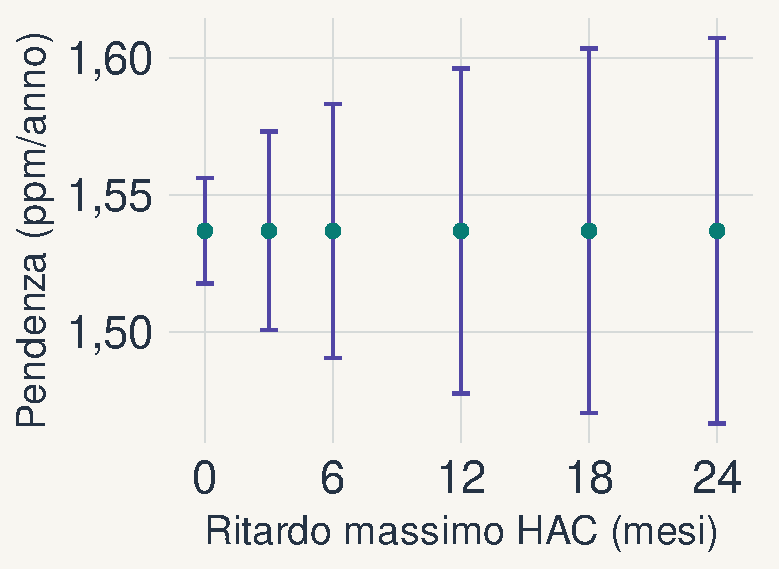
\includegraphics[width=\linewidth,height=6.15cm,keepaspectratio]{Figure/F07.pdf}\par}
\PSmall{Intervalli HAC lungo la griglia dichiarata di ritardi massimi; stima centrale OLS comune.}
}};
\node[anchor=north west,inner sep=0] at([xshift=10.85cm,yshift=-2.12cm]current page.north west){\Colonna{8.16cm}{\PBody{Il progetto confronta ritardi massimi di zero, tre, sei, dodici, diciotto e ventiquattro mesi, mantenendo invariati osservazioni e modello. Le ampiezze degli intervalli mostrano quanto la precisione dipenda dalla memoria inclusa nella covarianza. La griglia viene presentata integralmente, evitando di selezionare soltanto la costruzione più favorevole. Con dipendenza persistente, l’adeguatezza asintotica e la scelta del ritardo richiedono comunque una discussione: il confronto numerico delle varianti non elimina i limiti della serie finita.}
}};
\end{tikzpicture}\end{frame}

\begin{frame}[plain]\hypertarget{slide20}{}
\bookmark[level=0,page=20]{Curvatura, interpretazione e consegna}
\bookmark[level=1,page=20]{La curvatura modifica la forma della media}
\begin{tikzpicture}[remember picture,overlay]
\PilotChrome{La curvatura modifica la forma della media}{CURVATURA, INTERPRETAZIONE E CONSEGNA}{20}{La derivata collega la forma matematica del trend all’interpretazione del tasso locale.}
\node[anchor=north west,inner sep=0] at([xshift=.96cm,yshift=-2.12cm]current page.north west){\Colonna{9.40cm}{{\centering\resizebox{0.90\linewidth}{!}{\begin{tikzpicture}[x=1cm,y=-.87cm,every node/.style={font=\fontsize{12.2}{15}\selectfont,text=Ink},arr/.style={-{Stealth[length=2mm]},line width=.8pt,draw=Classical}]\path[use as bounding box] (0,0) rectangle (7.45,6.2);
\draw[Rule,line width=.8pt] (0.6,5.1)--(6.8,5.1);
\draw[Rule,line width=.8pt] (0.6,5.1)--(0.6,0.6);
\draw[Classical,line width=1pt] (.8,4.5)--(6.5,1.5);\draw[Quantum,line width=1.1pt] (.8,4.8) .. controls (3.2,4.5) and (4.7,3.1) .. (6.5,.9);\node[anchor=center,text=Ink,font=\fontsize{11}{15}\selectfont,text width=6.8cm,align=center] at (3.7,5.8) {Schema: pendenza costante e tasso variabile};
\node[anchor=center,text=Ink,font=\fontsize{11.5}{15}\selectfont,text width=6.7cm,align=center] at (3.7,0.25) {Forme della componente temporale};

\end{tikzpicture}}\par}
\PSmall{$\tau$: anni centrati nel 1993; m: mese; $\mu$: media in ppm; $\gamma_1=0$. $\beta_1$: ppm/anno; $\beta_2$: ppm/anno².}
}};
\node[anchor=north west,inner sep=0] at([xshift=10.85cm,yshift=-2.12cm]current page.north west){\Colonna{8.16cm}{\PBody{L’aggiunta del termine quadratico introduce una sensibilità descrittiva rispetto all’ipotesi di crescita lineare. Il suo coefficiente è circa 0,010174 ppm per anno quadrato, mentre il tasso locale diventa una funzione del tempo. Poiché il tempo è centrato, il coefficiente lineare del modello quadratico rappresenta il tasso al centro convenzionale e non una pendenza costante sull’intera finestra. La capacità predittiva su osservazioni future richiederebbe una valutazione ulteriore.}
\par\smallskip{\centering\adjustbox{max width=.98\linewidth}{$\displaystyle \begin{gathered}\mu(\tau,m)=\alpha+\beta_1\tau+\beta_2\tau^2+\gamma_m\\\frac{\partial\mu}{\partial\tau}=\beta_1+2\beta_2\tau\end{gathered}$}\par\smallskip}
}};
\end{tikzpicture}\end{frame}

\begin{frame}[plain]\hypertarget{slide21}{}
\bookmark[level=1,page=21]{La scala delle differenze fra adattamenti}
\begin{tikzpicture}[remember picture,overlay]
\PilotChrome{La scala delle differenze fra adattamenti}{CURVATURA, INTERPRETAZIONE E CONSEGNA}{21}{La rilevanza di una differenza fra modelli dipende dalla scala e dalla domanda scientifica.}
\node[anchor=north west,inner sep=0] at([xshift=.96cm,yshift=-2.12cm]current page.north west){\Colonna{9.40cm}{{\centering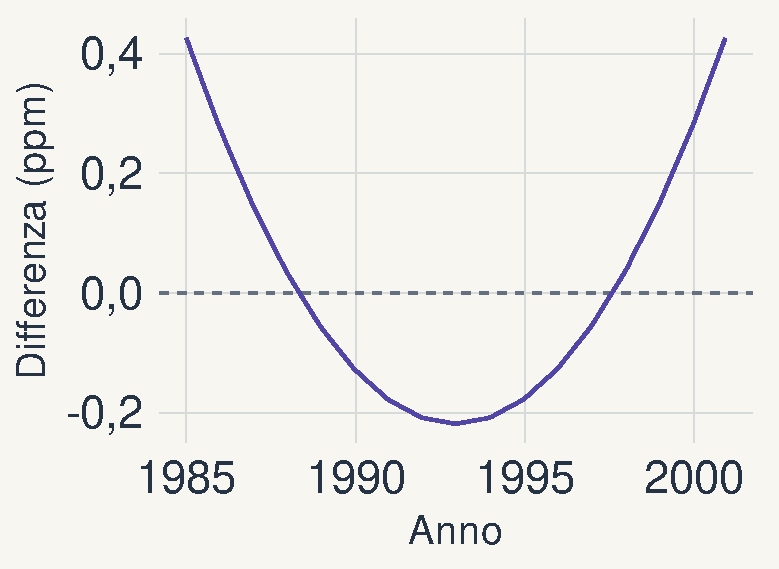
\includegraphics[width=\linewidth,height=6.15cm,keepaspectratio]{Figure/F08.pdf}\par}
\PSmall{Differenza fra i valori adattati dal modello quadratico e da quello lineare, in ppm.}
}};
\node[anchor=north west,inner sep=0] at([xshift=10.85cm,yshift=-2.12cm]current page.north west){\Colonna{8.16cm}{\PBody{La figura rappresenta il modello quadratico meno quello lineare, con la stessa parametrizzazione mensile e coefficienti ristimati. Lo scarto massimo in valore assoluto è circa 0,426 ppm, una grandezza piccola rispetto alla concentrazione complessiva ma pertinente alla forma della tendenza. La scala dedicata permette di esaminare questa differenza senza confonderla con il ciclo stagionale dominante. L’analisi considera la curvatura come sensibilità della media e non sceglie il modello in base alla convenienza di una probabilità di riferimento.}
}};
\end{tikzpicture}\end{frame}

\begin{frame}[plain]\hypertarget{slide22}{}
\bookmark[level=1,page=22]{Il tasso locale rende leggibile la conseguenza fisica}
\begin{tikzpicture}[remember picture,overlay]
\PilotChrome{{\fontsize{15.3}{19}\selectfont Il tasso locale rende leggibile la conseguenza fisica}}{CURVATURA, INTERPRETAZIONE E CONSEGNA}{22}{Un tasso locale viene interpretato nel dominio nel quale la funzione è stata stimata.}
\node[anchor=north west,inner sep=0] at([xshift=.96cm,yshift=-2.12cm]current page.north west){\Colonna{9.40cm}{{\centering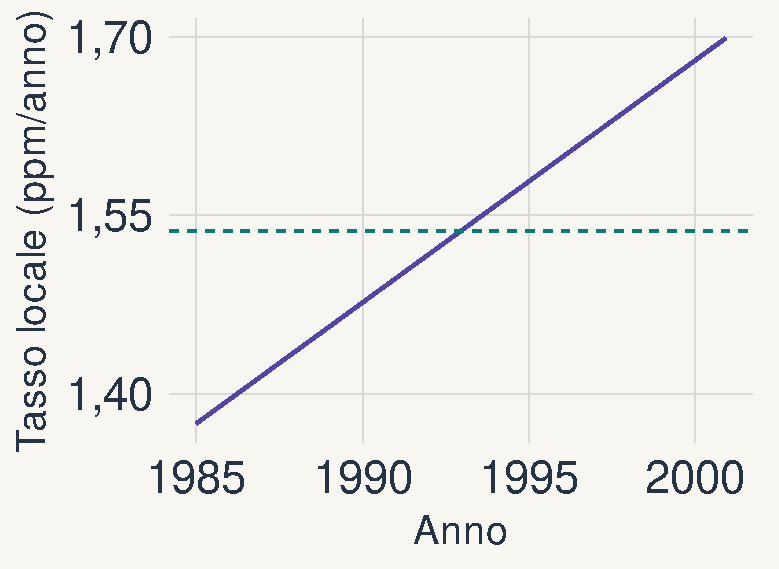
\includegraphics[width=\linewidth,height=6.15cm,keepaspectratio]{Figure/F09.pdf}\par}
\PSmall{Derivata temporale del modello quadratico. Riferimento tratteggiato: pendenza del modello lineare.}
}};
\node[anchor=north west,inner sep=0] at([xshift=10.85cm,yshift=-2.12cm]current page.north west){\Colonna{8.16cm}{\PBody{Nel modello quadratico, il tasso locale stimato varia da circa 1,375 a 1,699 ppm per anno lungo la finestra. Il riferimento tratteggiato riporta invece la pendenza costante del modello lineare, circa 1,537. La figura chiarisce che il coefficiente della curvatura modifica l’interpretazione della crescita nel tempo, pur lasciando il confronto entro lo stesso archivio storico. L’estrapolazione della parabola oltre il dominio osservato richiederebbe ulteriori ipotesi e una verifica su dati nuovi.}
}};
\end{tikzpicture}\end{frame}

\begin{frame}[plain]\hypertarget{slide23}{}
\bookmark[level=1,page=23]{Consegna: collegare copertura, trend e incertezza}
\begin{tikzpicture}[remember picture,overlay]
\PilotChrome{Consegna: collegare copertura, trend e incertezza}{CURVATURA, INTERPRETAZIONE E CONSEGNA}{23}{La sintesi finale conserva le scelte che determinano il significato della pendenza e della sua incertezza.}
\node[anchor=north west,inner sep=0] at([xshift=.96cm,yshift=-2.12cm]current page.north west){\Colonna{9.40cm}{\PBody{La relazione documenta fonte, conteggi mensili, finestra, modello stagionale, diagnosi dei residui e sensibilità della covarianza e della media. L’esercizio richiede di spiegare come un R² elevato possa convivere con un intervallo HAC più ampio, richiamando la differenza fra aderenza e dipendenza residua. Una seconda attività corregge un grafico che presenti le scatole stagionali come intervalli della pendenza. La conclusione riporta grandezza e unità del trend, mantenendo espliciti periodo, aggregazione e limiti dell’interpretazione fisica.}
}};
\node[anchor=north west,inner sep=0] at([xshift=10.85cm,yshift=-2.12cm]current page.north west){\Colonna{8.16cm}{\PInfo{R/P05\_figure.R ricostruisce medie, controlli, figure e confronti. R/covarianze.R contiene la formula HAC condivisa con P03. Il progetto raccorda descrizione temporale, regressione e previsione dei moduli M07, M09 e M10. L’aggiornamento richiede una nuova fonte e un audit completo delle definizioni.}
}};
\end{tikzpicture}\end{frame}

\begin{frame}[plain]\hypertarget{slide24}{}
\bookmark[level=0,page=24]{Laboratori della spedizione}
\bookmark[level=1,page=24]{Tre fasi della spedizione nel laboratorio}
\begin{tikzpicture}[remember picture,overlay]
\PilotChrome{Tre fasi della spedizione nel laboratorio}{LABORATORI DELLA SPEDIZIONE}{24}{Gli esperimenti usano serie sintetiche; la conclusione sul caso resta quella ottenuta dalle medie mensili di Mauna Loa.}
\node[anchor=north west,inner sep=0] at([xshift=.96cm,yshift=-2.12cm]current page.north west){\Colonna{9.40cm}{{\centering\resizebox{0.97\linewidth}{!}{\begin{tikzpicture}[x=1cm,y=1cm,every node/.style={font=\sffamily\fontsize{9.2}{11}\selectfont,text=Ink}]
\node[draw=Classical,fill=Classical,rounded corners=2mm,text=white,text width=2.45cm,align=flush center,minimum height=1.55cm,anchor=west,font=\sffamily\bfseries\fontsize{9.2}{11}\selectfont] (f0) at (0,0.00) {1. Conservare il tempo};
\node[draw=Classical!60,fill=Classical!6,rounded corners=1.5mm,line width=.6pt,text width=2.8cm,align=flush center,minimum height=1.55cm,anchor=west] (e00) at (2.95,0.00) {Calendario e osservazioni mancanti\\[1pt]{\fontsize{7.6}{9}\selectfont\color{Muted}m09-calendario}};
\node[draw=Rule,fill=white,rounded corners=1.5mm,line width=.6pt,text width=2.8cm,align=flush center,minimum height=1.55cm,anchor=west] (e01) at (6.10,0.00) {Risoluzione temporale e copertura\\[1pt]{\fontsize{7.6}{9}\selectfont\color{Muted}m09-aggregazione}};
\draw[pEdge] (f0.east)--(e00.west);
\node[draw=Classical,fill=Classical,rounded corners=2mm,text=white,text width=2.45cm,align=flush center,minimum height=1.55cm,anchor=west,font=\sffamily\bfseries\fontsize{9.2}{11}\selectfont] (f1) at (0,-1.95) {2. Separare le componenti};
\draw[pEdge] (f0.south)--(f1.north);
\node[draw=Classical!60,fill=Classical!6,rounded corners=1.5mm,line width=.6pt,text width=2.8cm,align=flush center,minimum height=1.55cm,anchor=west] (e10) at (2.95,-1.95) {Trend, stagionalità e media mobile\\[1pt]{\fontsize{7.6}{9}\selectfont\color{Muted}m09-smoothing}};
\node[draw=Rule,fill=white,rounded corners=1.5mm,line width=.6pt,text width=2.8cm,align=flush center,minimum height=1.55cm,anchor=west] (e11) at (6.10,-1.95) {Trasformazione e differenziazione\\[1pt]{\fontsize{7.6}{9}\selectfont\color{Muted}m09-differenze}};
\draw[pEdge] (f1.east)--(e10.west);
\node[draw=Classical,fill=Classical,rounded corners=2mm,text=white,text width=2.45cm,align=flush center,minimum height=1.55cm,anchor=west,font=\sffamily\bfseries\fontsize{9.2}{11}\selectfont] (f2) at (0,-3.90) {3. Confrontare previsioni};
\draw[pEdge] (f1.south)--(f2.north);
\node[draw=Classical!60,fill=Classical!6,rounded corners=1.5mm,line width=.6pt,text width=2.8cm,align=flush center,minimum height=1.55cm,anchor=west] (e20) at (2.95,-3.90) {Previsioni di riferimento e valutazione temporale\\[1pt]{\fontsize{7.6}{9}\selectfont\color{Muted}m10-riferimenti}};
\node[draw=Rule,fill=white,rounded corners=1.5mm,line width=.6pt,text width=2.8cm,align=flush center,minimum height=1.55cm,anchor=west] (e21) at (6.10,-3.90) {Struttura ARIMA e stagionalità\\[1pt]{\fontsize{7.6}{9}\selectfont\color{Muted}m10-arima}};
\draw[pEdge] (f2.east)--(e20.west);
\end{tikzpicture}
}\par}
\PSmall{Fasi della spedizione. Il primo esperimento di ogni fase ha le pagine Scenario A e Confronto.}
}};
\node[anchor=north west,inner sep=0] at([xshift=10.85cm,yshift=-2.12cm]current page.north west){\Colonna{8.16cm}{\PBody{Gli esperimenti ripetono su dati sintetici tre passaggi della spedizione: conservare il calendario, separare tendenza e stagionalità, confrontare previsioni di riferimento su un periodo successivo. Ogni fase ha uno scenario di partenza e un confronto con un solo parametro modificato.}
\vspace{.2cm}\PLabel{Altri esperimenti delle fasi}
\PLab{https://marzione00.github.io/Lab_Geo/\#laboratorio/m09-aggregazione}{Risoluzione temporale e copertura · m09-aggregazione}
\PLab{https://marzione00.github.io/Lab_Geo/\#laboratorio/m09-differenze}{Trasformazione e differenziazione · m09-differenze}
\PLab{https://marzione00.github.io/Lab_Geo/\#laboratorio/m10-arima}{Struttura ARIMA e stagionalità · m10-arima}
}};
\end{tikzpicture}\end{frame}

\begin{frame}[plain]\hypertarget{slide25}{}
\bookmark[level=1,page=25]{Calendario e osservazioni mancanti}
\begin{tikzpicture}[remember picture,overlay]
\PilotChrome{Calendario e osservazioni mancanti}{LABORATORI DELLA SPEDIZIONE}{25}{Distinguere distanza temporale e posizione nella tabella.}
\node[anchor=north west,inner sep=0] at([xshift=.96cm,yshift=-2.12cm]current page.north west){\Colonna{9.40cm}{{\centering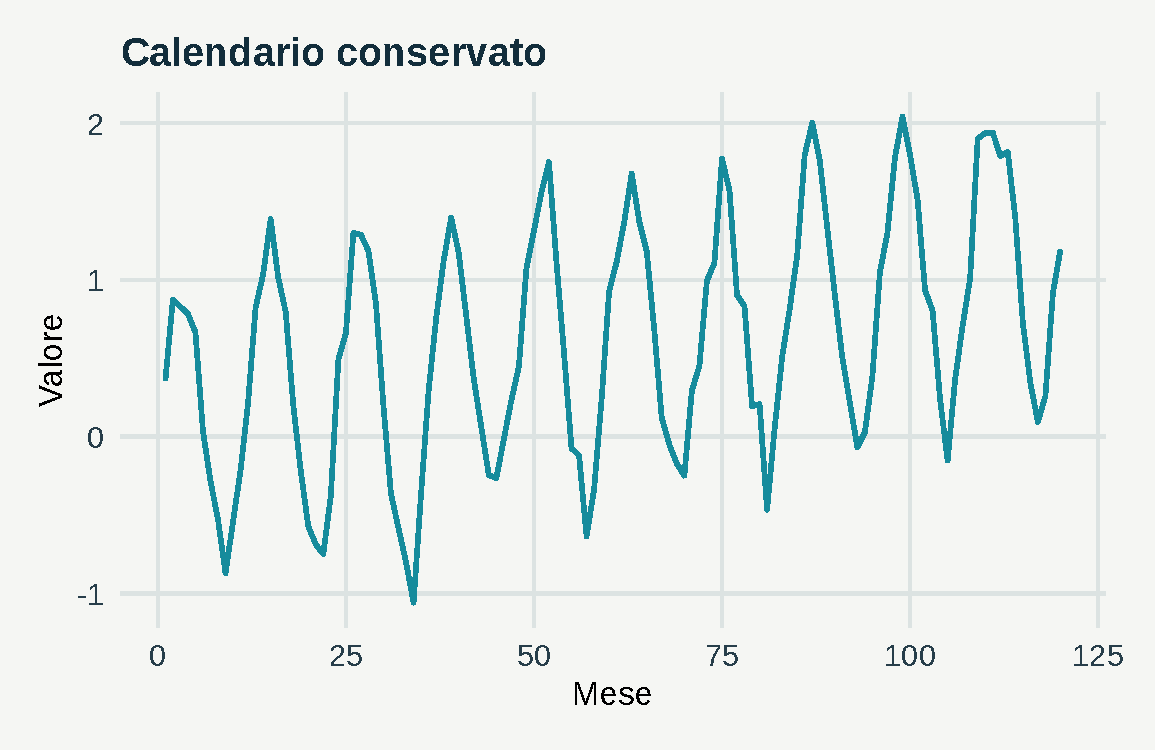
\includegraphics[width=\linewidth,height=5.0cm,keepaspectratio]{Esperimenti/m09-calendario-A.pdf}\par}
\PSmall{Mesi da escludere: 8. Seme: 17.}
\PSmall{$t_i$ è il mese della $i$-esima osservazione disponibile; $\Delta t_i$ è il tempo trascorso dalla precedente osservazione. In presenza di lacune, gli incrementi temporali possono essere maggiori di un mese.}
}};
\node[anchor=north west,inner sep=0] at([xshift=10.85cm,yshift=-2.12cm]current page.north west){\Colonna{8.16cm}{\PLabel{Scenario A · simulazione}
\PBody{La serie sintetica contiene una componente stagionale, un andamento di lungo periodo e rumore. Eliminando alcuni mesi si produce un insieme di osservazioni disponibili con intervalli temporali diseguali. Le date dei valori conservati rimangono note, consentendo di confrontare una rappresentazione che rispetta il calendario con una che utilizza soltanto la posizione nella tabella.}
\par\smallskip{\centering\adjustbox{max width=.98\linewidth}{$\displaystyle \Delta t_i=t_i-t_{i-1}$}\par\smallskip}
}};
\node[anchor=north east,inner sep=0] at([xshift=17.1cm,yshift=-12.04cm]current page.north west){\fontsize{7.7}{9}\selectfont \href{https://marzione00.github.io/Lab_Geo/\#laboratorio/m09-calendario}{\color{Classical}\bfseries Apri il laboratorio · m09-calendario}};
\end{tikzpicture}\end{frame}

\begin{frame}[plain]\hypertarget{slide26}{}
\bookmark[level=1,page=26]{Confronto | Calendario e osservazioni mancanti}
\begin{tikzpicture}[remember picture,overlay]
\PilotChrome{Confronto | Calendario e osservazioni mancanti}{LABORATORI DELLA SPEDIZIONE}{26}{L’indice di riga non sostituisce il calendario quando gli intervalli di osservazione sono irregolari.}
\node[anchor=north west,inner sep=0] at([xshift=.96cm,yshift=-2.12cm]current page.north west){\Colonna{9.40cm}{{\centering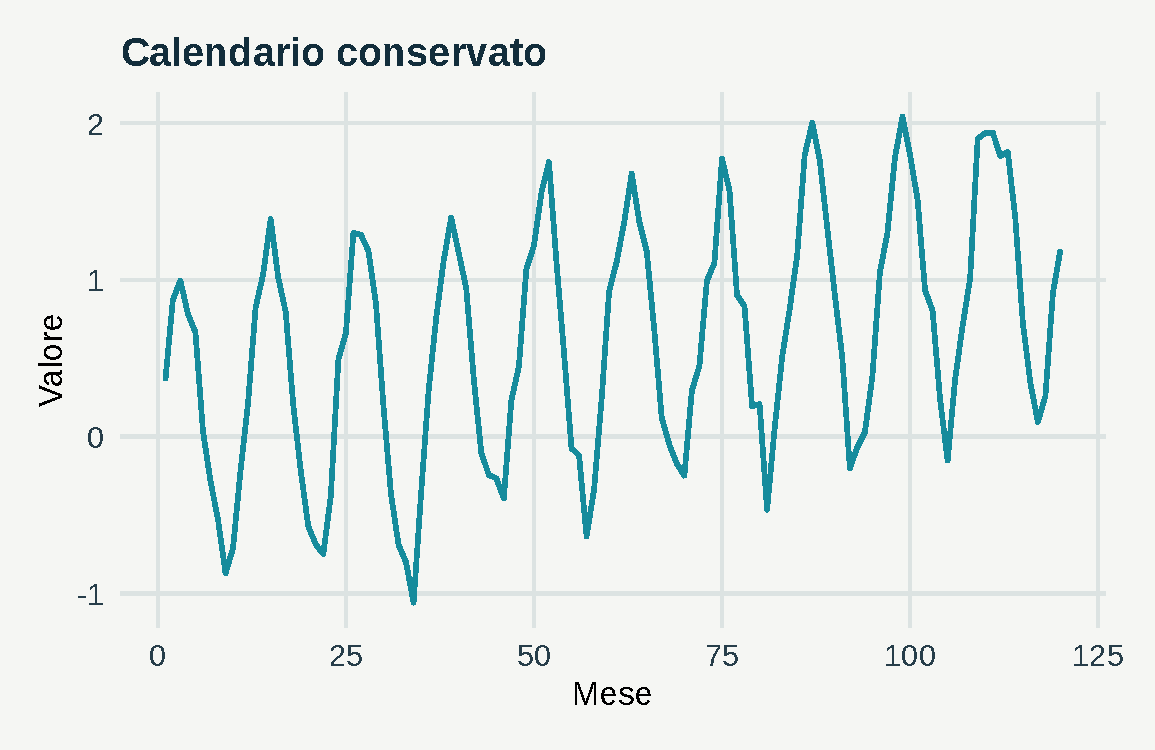
\includegraphics[width=\linewidth,height=5.6cm,keepaspectratio]{Esperimenti/m09-calendario-B.pdf}\par}
\PSmall{Mesi da escludere: 8 $\to$ 0. Tutti gli altri parametri e il seme sono fissi.}
}};
\node[anchor=north west,inner sep=0] at([xshift=10.85cm,yshift=-2.12cm]current page.north west){\Colonna{8.16cm}{\PLabel{Confronto fra gli scenari}
{\fontsize{10.2}{12.8}\selectfont\begin{tabular}{@{}>{\raggedright\arraybackslash}p{0.48\linewidth}@{\hspace{.13cm}}>{\raggedright\arraybackslash}p{0.224\linewidth}@{\hspace{.13cm}}>{\raggedright\arraybackslash}p{0.224\linewidth}@{}}\toprule Grandezza & A & B\\[2.3pt]
\midrule 
Osservazioni & 112 & 120\\[2.3pt]
Intervallo massimo fra osservazioni & 2 & 1\\[2.3pt]
\bottomrule\end{tabular}\par}
\vspace{.25cm}\PBody{Senza mesi esclusi le osservazioni salgono da 112 a 120 e l’intervallo massimo torna a un mese. Nella spedizione il conteggio delle settimane valide precede la scelta della finestra, così ogni media mensile ha un denominatore dichiarato.}
}};
\node[anchor=north east,inner sep=0] at([xshift=17.1cm,yshift=-12.04cm]current page.north west){\fontsize{7.7}{9}\selectfont \href{https://marzione00.github.io/Lab_Geo/\#laboratorio/m09-calendario}{\color{Classical}\bfseries Apri il laboratorio · m09-calendario}};
\end{tikzpicture}\end{frame}

\begin{frame}[plain]\hypertarget{slide27}{}
\bookmark[level=1,page=27]{Trend, stagionalità e media mobile}
\begin{tikzpicture}[remember picture,overlay]
\PilotChrome{Trend, stagionalità e media mobile}{LABORATORI DELLA SPEDIZIONE}{27}{Confrontare componenti note e stima mediante smoothing.}
\node[anchor=north west,inner sep=0] at([xshift=.96cm,yshift=-2.12cm]current page.north west){\Colonna{9.40cm}{{\centering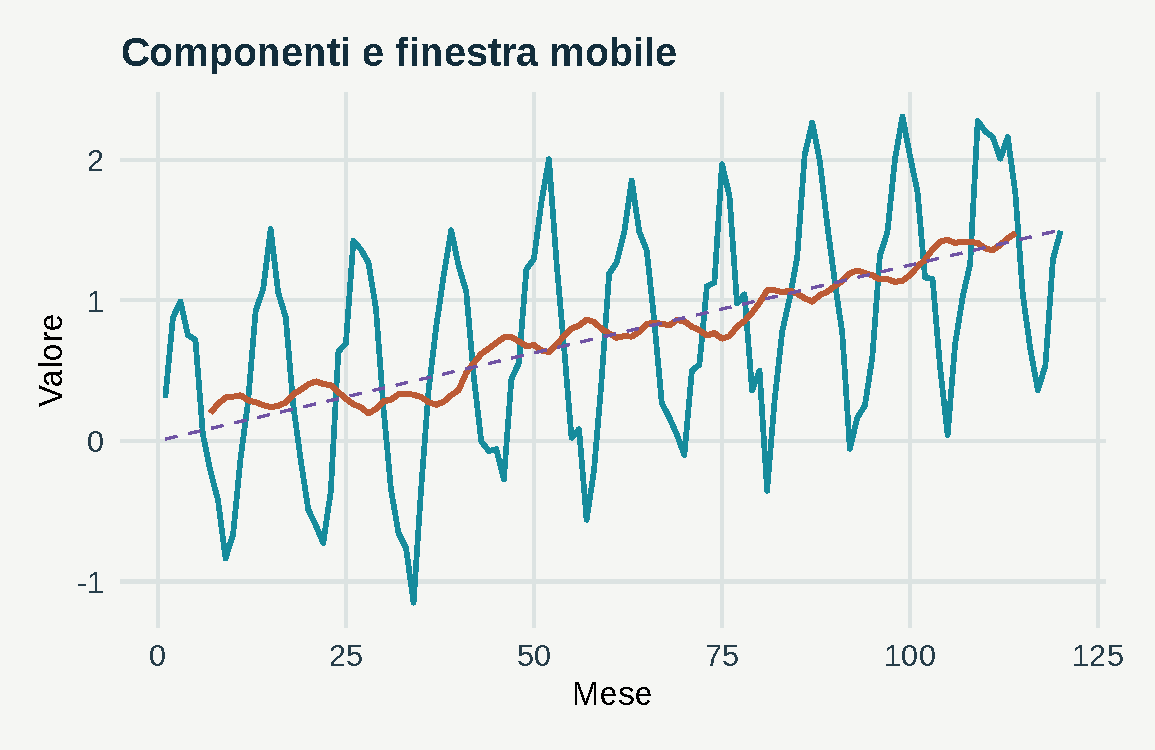
\includegraphics[width=\linewidth,height=5.0cm,keepaspectratio]{Esperimenti/m09-smoothing-A.pdf}\par}
\PSmall{Semilarghezza della finestra: 6. Seme: 17.}
\PSmall{$x_t$ è la serie osservata; $k$ è la semilarghezza della finestra, che contiene $2k+1$ mesi. $\widehat m_t$ è la media mobile centrata al tempo $t$, definita quando tutte le osservazioni della finestra sono disponibili.}
}};
\node[anchor=north west,inner sep=0] at([xshift=10.85cm,yshift=-2.12cm]current page.north west){\Colonna{8.16cm}{\PLabel{Scenario A · simulazione}
\PBody{Il segnale viene costruito sommando un trend lineare, una componente stagionale e un errore casuale. La media mobile centrata utilizza un numero dispari di osservazioni, collocate simmetricamente rispetto al tempo rappresentato. Modificando la semilarghezza della finestra si può esaminare il compromesso fra regolarizzazione del segnale e conservazione delle oscillazioni.}
\par\smallskip{\centering\adjustbox{max width=.98\linewidth}{$\displaystyle \widehat m_t=\frac1{2k+1}\sum_{j=-k}^{k}x_{t+j}$}\par\smallskip}
}};
\node[anchor=north east,inner sep=0] at([xshift=17.1cm,yshift=-12.04cm]current page.north west){\fontsize{7.7}{9}\selectfont \href{https://marzione00.github.io/Lab_Geo/\#laboratorio/m09-smoothing}{\color{Classical}\bfseries Apri il laboratorio · m09-smoothing}};
\end{tikzpicture}\end{frame}

\begin{frame}[plain]\hypertarget{slide28}{}
\bookmark[level=1,page=28]{Confronto | Trend, stagionalità e media mobile}
\begin{tikzpicture}[remember picture,overlay]
\PilotChrome{Confronto | Trend, stagionalità e media mobile}{LABORATORI DELLA SPEDIZIONE}{28}{La finestra definisce la scala temporale della sintesi; i bordi richiedono una convenzione esplicita.}
\node[anchor=north west,inner sep=0] at([xshift=.96cm,yshift=-2.12cm]current page.north west){\Colonna{9.40cm}{{\centering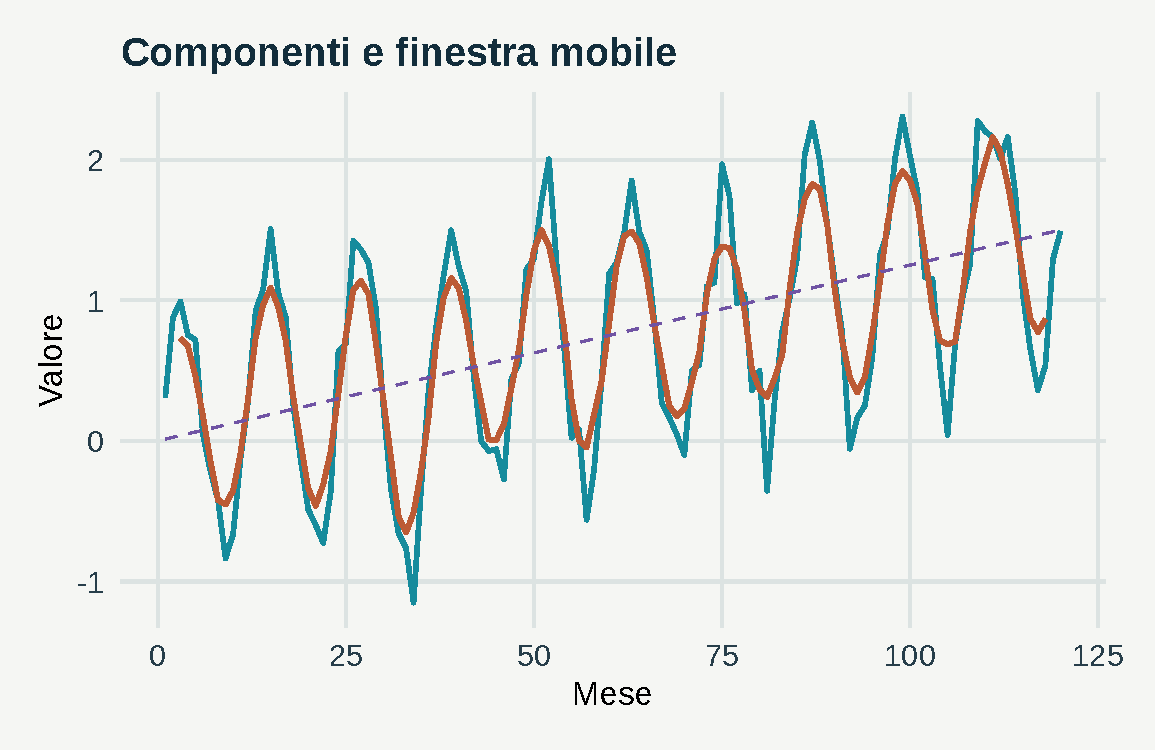
\includegraphics[width=\linewidth,height=5.6cm,keepaspectratio]{Esperimenti/m09-smoothing-B.pdf}\par}
\PSmall{Semilarghezza della finestra: 6 $\to$ 2. Tutti gli altri parametri e il seme sono fissi.}
}};
\node[anchor=north west,inner sep=0] at([xshift=10.85cm,yshift=-2.12cm]current page.north west){\Colonna{8.16cm}{\PLabel{Confronto fra gli scenari}
{\fontsize{10.2}{12.8}\selectfont\begin{tabular}{@{}>{\raggedright\arraybackslash}p{0.48\linewidth}@{\hspace{.13cm}}>{\raggedright\arraybackslash}p{0.224\linewidth}@{\hspace{.13cm}}>{\raggedright\arraybackslash}p{0.224\linewidth}@{}}\toprule Grandezza & A & B\\[2.3pt]
\midrule 
Ampiezza finestra & 13 & 5\\[2.3pt]
Valori senza finestra completa & 12 & 4\\[2.3pt]
RMSE rispetto al trend & 0,0997 & 0,533\\[2.3pt]
\bottomrule\end{tabular}\par}
\vspace{.25cm}\PBody{Con semilarghezza 2 la finestra passa da 13 a 5 mesi e i valori senza finestra completa da 12 a 4, mentre lo scarto dal trend sale da 0,0997 a 0,533. Una finestra più corta di un anno lascia passare l’oscillazione stagionale.}
}};
\node[anchor=north east,inner sep=0] at([xshift=17.1cm,yshift=-12.04cm]current page.north west){\fontsize{7.7}{9}\selectfont \href{https://marzione00.github.io/Lab_Geo/\#laboratorio/m09-smoothing}{\color{Classical}\bfseries Apri il laboratorio · m09-smoothing}};
\end{tikzpicture}\end{frame}

\begin{frame}[plain]\hypertarget{slide29}{}
\bookmark[level=1,page=29]{Previsioni di riferimento e valutazione temporale}
\begin{tikzpicture}[remember picture,overlay]
\PilotChrome{Previsioni di riferimento e valutazione temporale}{LABORATORI DELLA SPEDIZIONE}{29}{Confrontare media, ultimo valore e riferimento stagionale.}
\node[anchor=north west,inner sep=0] at([xshift=.96cm,yshift=-2.12cm]current page.north west){\Colonna{9.40cm}{{\centering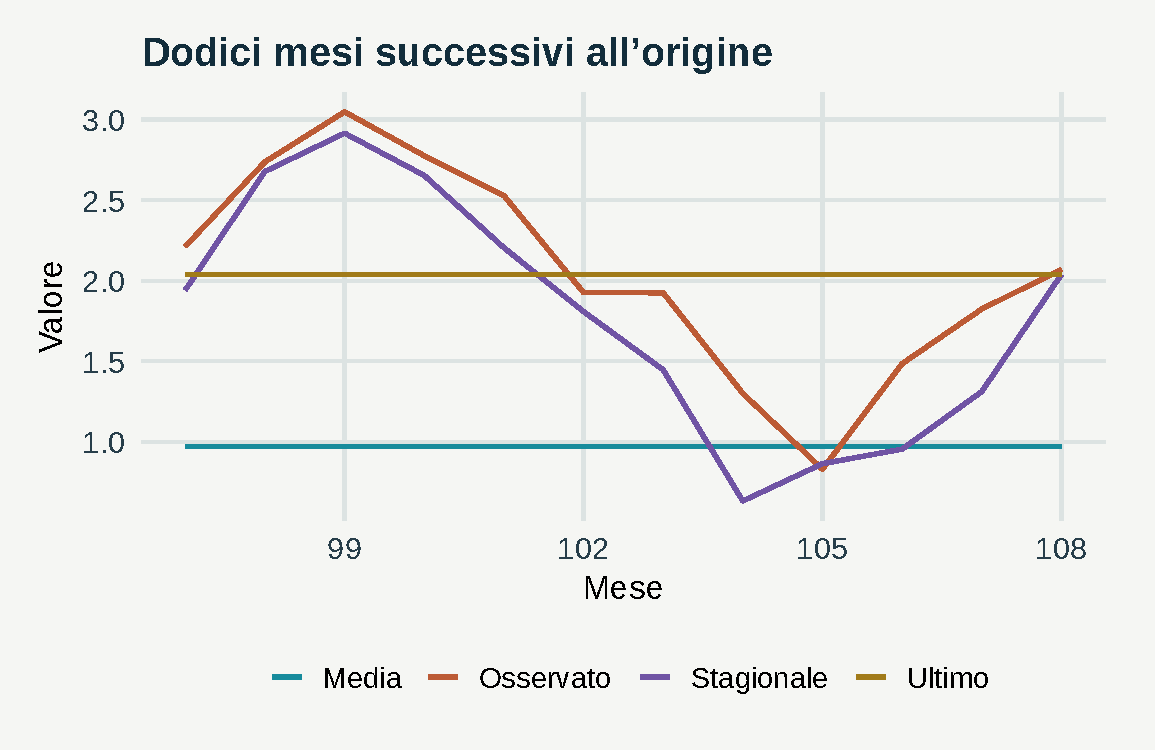
\includegraphics[width=\linewidth,height=5.0cm,keepaspectratio]{Esperimenti/m10-riferimenti-A.pdf}\par}
\PSmall{Ultimo mese disponibile: 96. Seme: 17.}
\PSmall{$t$ è l’origine della previsione; $H$ è il numero di passi valutati; $y_{t+h}$ è il valore osservato e $\widehat y_{t+h}$ la previsione. MAE è la media degli errori assoluti e mantiene l’unità della serie.}
}};
\node[anchor=north west,inner sep=0] at([xshift=10.85cm,yshift=-2.12cm]current page.north west){\Colonna{8.16cm}{\PLabel{Scenario A · simulazione}
\PBody{Una serie con trend, stagionalità annuale e rumore viene divisa in corrispondenza dell’origine scelta. Le previsioni per i dodici mesi successivi utilizzano tre riferimenti: media del passato, ultima osservazione e valori dei dodici mesi precedenti. Tutti i procedimenti dispongono soltanto delle informazioni anteriori o contemporanee all’origine.}
\par\smallskip{\centering\adjustbox{max width=.98\linewidth}{$\displaystyle \operatorname{MAE}=H^{-1}\sum_h|y_{t+h}-\widehat y_{t+h}|$}\par\smallskip}
}};
\node[anchor=north east,inner sep=0] at([xshift=17.1cm,yshift=-12.04cm]current page.north west){\fontsize{7.7}{9}\selectfont \href{https://marzione00.github.io/Lab_Geo/\#laboratorio/m10-riferimenti}{\color{Classical}\bfseries Apri il laboratorio · m10-riferimenti}};
\end{tikzpicture}\end{frame}

\begin{frame}[plain]\hypertarget{slide30}{}
\bookmark[level=1,page=30]{Confronto | Previsioni di riferimento e valutazione temporale}
\begin{tikzpicture}[remember picture,overlay]
\PilotChrome{{\fontsize{15.3}{19}\selectfont Confronto | Previsioni di riferimento e valutazione temporale}}{LABORATORI DELLA SPEDIZIONE}{30}{La valutazione deve riprodurre l’informazione accessibile al momento della previsione.}
\node[anchor=north west,inner sep=0] at([xshift=.96cm,yshift=-2.12cm]current page.north west){\Colonna{9.40cm}{{\centering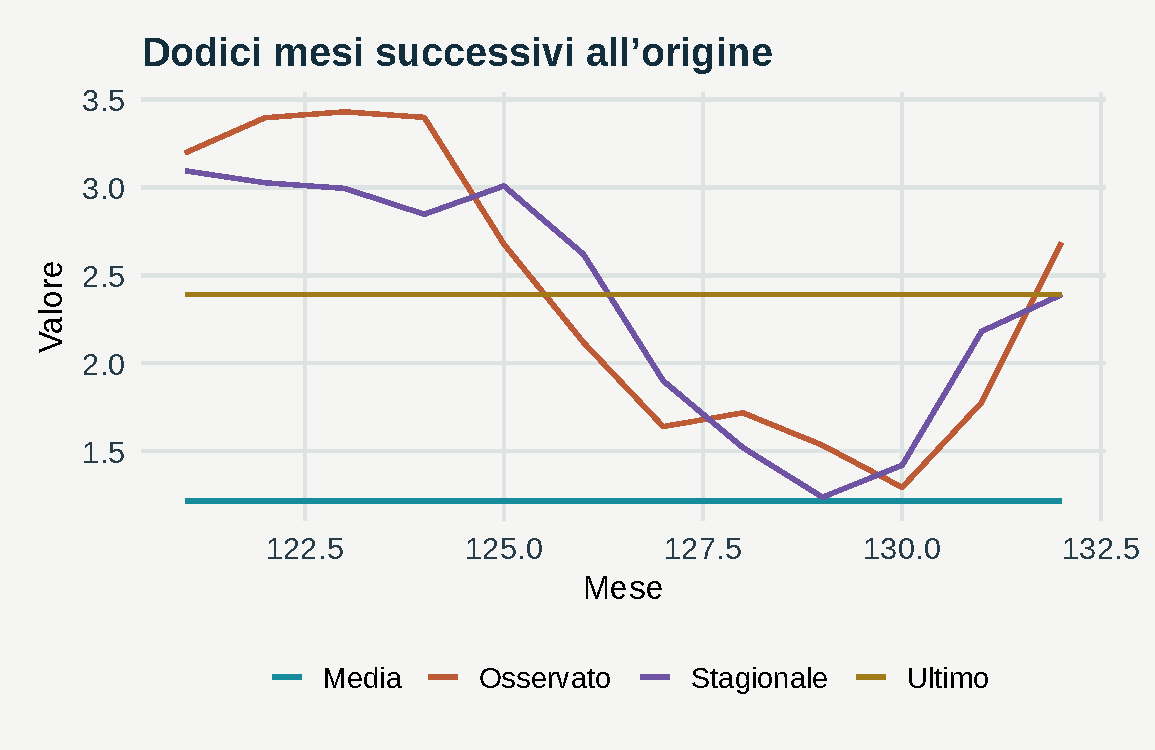
\includegraphics[width=\linewidth,height=5.6cm,keepaspectratio]{Esperimenti/m10-riferimenti-B.pdf}\par}
\PSmall{Ultimo mese disponibile: 96 $\to$ 120. Tutti gli altri parametri e il seme sono fissi.}
}};
\node[anchor=north west,inner sep=0] at([xshift=10.85cm,yshift=-2.12cm]current page.north west){\Colonna{8.16cm}{\PLabel{Confronto fra gli scenari}
{\fontsize{10.2}{12.8}\selectfont\begin{tabular}{@{}>{\raggedright\arraybackslash}p{0.48\linewidth}@{\hspace{.13cm}}>{\raggedright\arraybackslash}p{0.224\linewidth}@{\hspace{.13cm}}>{\raggedright\arraybackslash}p{0.224\linewidth}@{}}\toprule Grandezza & A & B\\[2.3pt]
\midrule 
MAE media & 1,11 & 1,19\\[2.3pt]
MAE ultimo & 0,507 & 0,725\\[2.3pt]
MAE stagionale & 0,274 & 0,322\\[2.3pt]
\bottomrule\end{tabular}\par}
\vspace{.25cm}\PBody{Spostando l’ultimo mese disponibile da 96 a 120 cambiano gli errori assoluti medi di tutti i riferimenti, e la previsione stagionale resta la migliore, da 0,274 a 0,322. Il confronto fra metodi va ripetuto su più origini per separarlo dal periodo valutato.}
}};
\node[anchor=north east,inner sep=0] at([xshift=17.1cm,yshift=-12.04cm]current page.north west){\fontsize{7.7}{9}\selectfont \href{https://marzione00.github.io/Lab_Geo/\#laboratorio/m10-riferimenti}{\color{Classical}\bfseries Apri il laboratorio · m10-riferimenti}};
\end{tikzpicture}\end{frame}

\begin{frame}[plain]\hypertarget{slide31}{}
\bookmark[level=1,page=31]{Dal risultato alla relazione}
\begin{tikzpicture}[remember picture,overlay]
\PilotChrome{Dal risultato alla relazione}{SINTESI}{31}{Riporta tasso, unità, finestra, aggregazione e intervallo HAC con il ritardo massimo dichiarato.}
\node[anchor=north west,inner sep=0] at([xshift=.96cm,yshift=-2.12cm]current page.north west){\Colonna{9.40cm}{\PLabel{Domanda di partenza}
\PBody{Quale tendenza si stima a Mauna Loa fra il 1985 e il 2000, al netto del calendario stagionale?}
\PLabel{Risultato da discutere}
\PBody{La pendenza stimata è circa 1,537 ppm per anno, con intervallo HAC da 1,478 a 1,596, più ampio di quello classico da 1,514 a 1,559 per la dipendenza residua. Con un termine quadratico il tasso locale cresce da circa 1,375 a 1,699 ppm per anno lungo la finestra.}
}};
\node[anchor=north west,inner sep=0] at([xshift=10.85cm,yshift=-2.12cm]current page.north west){\Colonna{8.16cm}{\PLabel{Limiti della conclusione}
\PBody{Il risultato riguarda sedici anni di medie mensili derivate da dati settimanali storici. L’estrapolazione della curvatura oltre il dominio osservato e il confronto con dati ufficiali aggiornati richiedono una nuova ricostruzione del protocollo.}
\vspace{.4cm}\href{https://marzione00.github.io/Lab_Geo/\#modulo-P06}{\color{Classical}\bfseries Prosegui · P06 · Dai campioni alla validazione spaziale}
}};
\end{tikzpicture}\end{frame}

\begin{frame}[plain]\hypertarget{slide32}{}
\bookmark[level=1,page=32]{Fonti, dati e codice per riprodurre le figure}
\begin{tikzpicture}[remember picture,overlay]
\PilotChrome{Fonti, dati e codice per riprodurre le figure}{RIFERIMENTI}{32}{I risultati numerici si riferiscono ai dati e alle ipotesi dichiarate nel caso.}
\node[anchor=north west,inner sep=0] at([xshift=.96cm,yshift=-2.12cm]current page.north west){\Colonna{9.40cm}{\PLabel{Dati e attribuzioni}
\PBody{Serie storica della CO$_2$ a Mauna Loa (Keeling e Whorf, 2004, tramite CDIAC), nella versione settimanale distribuita con statsmodels; le medie mensili sono derivate nella spedizione.}
}};
\node[anchor=north west,inner sep=0] at([xshift=10.85cm,yshift=-2.12cm]current page.north west){\Colonna{8.16cm}{\PLabel{Nell’archivio dei sorgenti}
\PBody{Codice contiene i frammenti delle pagine; R contiene lo script P05\_figure.R, che ricostruisce figure e valori dai dati. Esperimenti comprende i programmi dei due scenari, Diagrammi i disegni TikZ modificabili, Scena il modello Blender della copertina.}
\vspace{.4cm}\href{https://marzione00.github.io/Lab_Geo/\#modulo-P05}{\color{Classical}\bfseries Apri la spedizione P05 su GeoStat Lab}
}};
\end{tikzpicture}\end{frame}
\end{document}
